% !Mode:: "TeX:UTF-8"
%!TEX program = xelatex


\documentclass[a4paper,12pt,UTF8]{ctexart}
%\documentclass[a4paper,12pt]{article}%A4纸,正文为小四号字,对应12pt

\usepackage{titletoc}%自定义目录页样式
%\usepackage[UTF8]{ctex}


\usepackage{picinpar,graphicx}%图像 
\usepackage{subfig}%组合图像
\graphicspath{{插图/}}%表示在该目录下存放有一个图片

\usepackage{hyperref}%超链接宏包
\usepackage{enumerate}%用于列表环境自定义编号
\usepackage{titlesec}%改变章节编号形式

\usepackage{bm}%粗黑斜体的宏包,可以很方便表示矢量
\usepackage{amsmath}%数学公式换行、对齐
\usepackage{textcomp,gensymb}%调用常用的数学符号
\usepackage{amssymb}%调用常用的数学符号

\usepackage{tikz}

\usepackage{color}%设置字体颜色

\usepackage{datetime}%读取系统时间


\begin{document}
%--------------- 目录页格式定制 ---------------
\titlecontents{section}
	[0em]
	{\bf}
	{\contentslabel{2em}}
	{}
	{\titlerule*[1em]{$\cdot$}\contentspage}
\setcounter{tocdepth}{1}

%--------------- 章节编号形式定制 ---------------
\titleformat{\section}{\centering\Huge\bfseries}{第\,\thesection\,章}{1em}{}



% ----------- 封面 ---------------
\begin{center}  % 居中
\quad \\
\vspace{1cm}  % 间距
\heiti{\Huge{{《伯克利物理学教程》\textcolor[rgb]{1,0,1}{(力学卷)}\par 答案解析}}} \\
\vspace{1cm}
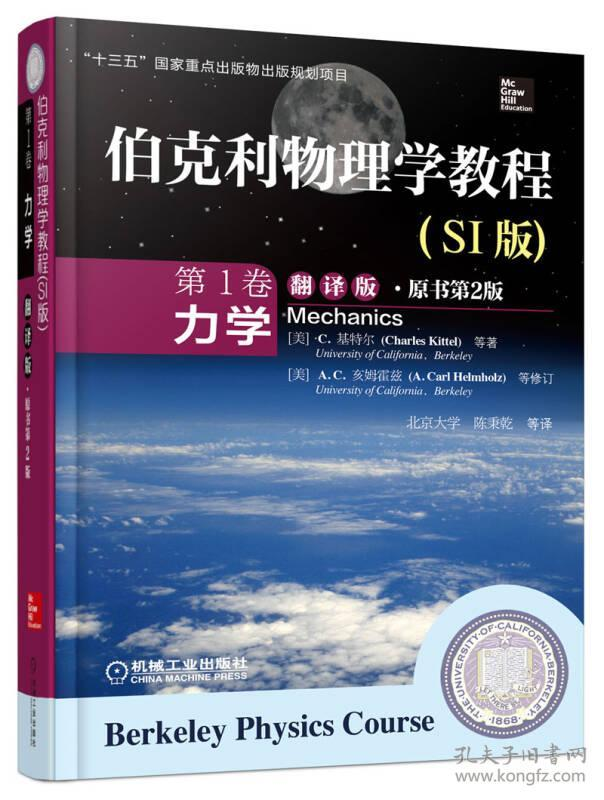
\includegraphics[width=0.65\textwidth]{伯克利物理学教程(力学).jpg} \\
\vspace{1cm}
\Large {\xxivtime \, \today} \\
%\Large{\renewcommand{\today}{\number\year 年 \number\month 月 \number\day 日}\today} \\
\vspace{0.5cm}
蓝天龙
\thispagestyle{empty}
\end{center}



%正文
\newpage
\tableofcontents\setcounter{page}{0} \thispagestyle{empty}

\clearpage
%!TeX root =main.tex
%!TEX program = XeLaTeX
% !Mode:: "TeX:UTF-8"

\section{绪论}

我好像没有做第一章的习题……

\clearpage
%!TeX root =main.tex
 %!TEX program = XeLaTeX
% !Mode:: "TeX:UTF-8"


\section{矢量}

\subsection{位置矢量}
\begin{enumerate}[(a)]
%%%%%%  1.1 题  %%%%%%%%%%%%%%	
	\item
	因为是东北方向,即矢量$\bm{r}$ 与x轴正方向、y轴正方向的夹角均为45\degree,所以矢量$\bm{r}$在x轴、y轴上的投影大小是一样的。即$r_x = r_y$,\\
所以有
		$$ {r_x}^2 + {r_y}^2 = 2 {r_x}^2 = 10^2 $$
		$$  x = 5\sqrt{2} = y $$
因此
		$$ \bm{r} = 5 \sqrt{2} \hat{\bm{x}} + 5 \sqrt{2} \hat{\bm{y}} + 2 \hat{\bm{z}} $$
		$$ \lvert{\bm{r}}\rvert = \sqrt{\sqrt{50}^2 + \sqrt{50}^2 + 2^2} = \sqrt{104} $$
		
		设$\bm{r} $的方向为 $ \hat{\bm{r}} = A\hat{\bm{x}} + B\hat{\bm{y}} + C\hat{\bm{z}} $ ,\\
		则有
		\[
		 \left\{
		 \begin{aligned}
		&\frac{B}{A} = 1 \\
		&\frac{C}{A} = \frac{\sqrt{2}}{5} \\
		&A^2+B^2+C^2 = 1^2
		 \end{aligned}
		 \right.
		 \Rightarrow \quad
		\left\{
		 \begin{aligned}
		&A = \frac{5}{\sqrt{52}} \\
		&B = \frac{5}{\sqrt{52}} \\
		&C = \sqrt{\frac{2}{52}}
		 \end{aligned}
		 \right.
		\]

%%%%%%  1.2 题  %%%%%%%%%%%%%%

	\item
	因为是东南方向,即矢量$\bm{r}$ 与x轴正方向、y轴负方向的夹角均为45\degree,所以矢量$\bm{r}$在x轴、y轴上的投影大小相等,方向相反。即$r_x = -r_y$,\\
所以有
		$$ {r_x}^2 + {r_y}^2 = 2 {r_x}^2 = 5^2 $$
		$$  x = \frac{5\sqrt{2}}{2} $$
		$$  y = -\frac{5\sqrt{2}}{2} $$
因此
		$$ \bm{r} =\frac{5\sqrt{2}}{2} \hat{\bm{x}} -\frac{5\sqrt{2}}{2} \hat{\bm{y}} - 5 \hat{\bm{z}} $$
		$$ \lvert{\bm{r}}\rvert = \sqrt{{\frac{5\sqrt{2}}{2}}^2 +{\frac{5\sqrt{2}}{2}}^2 + {-5}^2} = 5\sqrt{2} $$
		
		设$\bm{r} $的方向为 $ \hat{\bm{r}} = A\hat{\bm{x}} + B\hat{\bm{y}} + C\hat{\bm{z}} $ ,\\
		则有
		\[
		 \left\{
		 \begin{aligned}
		&\frac{B}{A} = -1 \\
		&\frac{C}{A} =-\sqrt{2} \\
		&A^2+B^2+C^2 = 1^2
		 \end{aligned}
		 \right.
		 \Rightarrow \quad
		\left\{
		 \begin{aligned}
		&A = \frac{1}{2} \\
		&B = -\frac{1}{2} \\
		&C = -\frac{\sqrt{2}}{2}
		 \end{aligned}
		 \right.
		\]
		
%%%%%%  1.3 题  %%%%%%%%%%%%%%	
		
	\item
	因为是西北方向,即矢量$\bm{r}$ 与x轴负方向、y轴正方向的夹角均为45\degree,所以矢量$\bm{r}$在x轴、y轴上的投影大小相等,方向相反。即$-r_x = r_y$,\\
所以有
		$$ {r_x}^2 + {r_y}^2 = 2 {r_y}^2 = 1^2 $$
		$$  x = -\frac{\sqrt{2}}{2} $$
		$$  y = \frac{\sqrt{2}}{2} $$
因此
		$$ \bm{r} =-\frac{\sqrt{2}}{2} \hat{\bm{x}} + \frac{\sqrt{2}}{2} \hat{\bm{y}} + 6 \hat{\bm{z}} $$
		$$ \lvert{\bm{r}}\rvert = \sqrt{{-\frac{\sqrt{2}}{2}}^2 +{\frac{\sqrt{2}}{2}}^2 + 6^2} = \sqrt{37} $$
		
		设$\bm{r} $的方向为 $ \hat{\bm{r}} = A\hat{\bm{x}} + B\hat{\bm{y}} + C\hat{\bm{z}} $ ,\\
		则有
		\[
		 \left\{
		 \begin{aligned}
		&\frac{B}{A} = -1 \\
		&\frac{C}{A} =-6 \sqrt{2} \\
		&A^2+B^2+C^2 = 1^2
		 \end{aligned}
		 \right.
		 \Rightarrow \quad
		\left\{
		 \begin{aligned}
		&A = -\frac{1}{\sqrt{74}} \\
		&B = \frac{1}{\sqrt{74}} \\
		&C = 12\sqrt{37}
		 \end{aligned}
		 \right.
		\]
\end{enumerate}
%%%
%%%
%%%
%%%
%%%
\subsection{矢量的分量}
\begin{enumerate}[(a)]
%%%%%% 2.1 题  %%%%%%%%%%%%%%	
	\item
	因为是东南方向,即矢量$\bm{r}$ 与x轴正方向、y轴负方向的夹角均为45\degree,所以矢量$\bm{r}$在x轴、y轴上的投影大小相等,方向相反。即$r_x = -r_y$,\\
所以有
		$$ {r_x}^2 + {r_y}^2 = 2 {r_x}^2 = 5^2 $$
		$$  x = \frac{5\sqrt{2}}{2} $$
		$$  y = -\frac{5\sqrt{2}}{2} $$
因此
		$$ \bm{r} =\frac{5\sqrt{2}}{2} \hat{\bm{x}} -\frac{5\sqrt{2}}{2} \hat{\bm{y}} $$
		
		
%%%%%%  2.2 题  %%%%%%%%%%%%%%		
	\item
	因为位置矢量$\bm{r}$与铅直线方向,即z轴的夹角为45\degree,水平分量方向为北60\degree 西,所以,设位置矢量$\bm{r} = -A\hat{\bm{x}} + B\hat{\bm{y}} + C\hat{\bm{z}}$,其中,$A,  B,  C$均为实数,且A,B,C应该满足的关系
		\[
		\left\{
		\begin{aligned}
		&\frac{B}{A} = -\sin 60\degree = - \frac{\sqrt{3}}{2} \\
		&\frac{\sqrt{A^2+B^2}}{C} =\cos 45\degree=-\frac{\sqrt{2}}{2} \\
		&\sqrt{A^2+B^2+C^2} = 15
		\end{aligned}
		\right.
		 \Rightarrow \quad
		\left\{
		 \begin{aligned}
		&A = -\sqrt{\frac{300}{7}} \\
		&B = \sqrt{\frac{225}{7}} \\
		&C = 5\sqrt{6}
		 \end{aligned}
		 \right.
		\]
即 位置矢量$\bm{r} = -\sqrt{\frac{300}{7}} \hat{\bm{x}} + \sqrt{\frac{225}{7}} \hat{\bm{y}} +5\sqrt{6} \hat{\bm{z}}$
\end{enumerate}
%%%
%%%
%%%
%%%
%%%
\subsection{矢量的相加}
\begin{enumerate}[(a)]
	\item 如下图(\ref{2_3a})所示。
	\item 如下图(\ref{2_3b})所示。
	\item 如下图(\ref{2_3c})所示。当一对矢量为另一对矢量的倍数时,不妨设为$ m $倍,则这对矢量相加的结果为另一对矢量相加结果的$ m $倍。证明如下:

设
	\[
	\begin{aligned}
	&\bm{a} = (x_1,y_1), \bm{b} = (x_2,y_2), \\
	&\bm{c} = m\bm{a} = (mx_1,my_1), \\
	&\bm{d} = m\bm{b} = (m x_2,m y_2).\\
	\end{aligned}
	 \]
则有
	\[
	\begin{aligned}
	\bm{g} &= \bm{a} + \bm{b} = (x_1 + x_2, y_1+y_2).\\
	\bm{h} &= \bm{c} + \bm{d} \\
			&= (mx_1 + mx_2, my_1 + my_2) \\
			&=m(x_1+x_2, y_1+y_2) \\
			&=m\bm{g}
	\end{aligned}
	\]
证毕。
\end{enumerate}

%%%%以下画图时间
\begin{figure}[htbp]
	\centering
	\subfloat[]{
	\begin{minipage}[t]{0.5\linewidth}
	\centering
	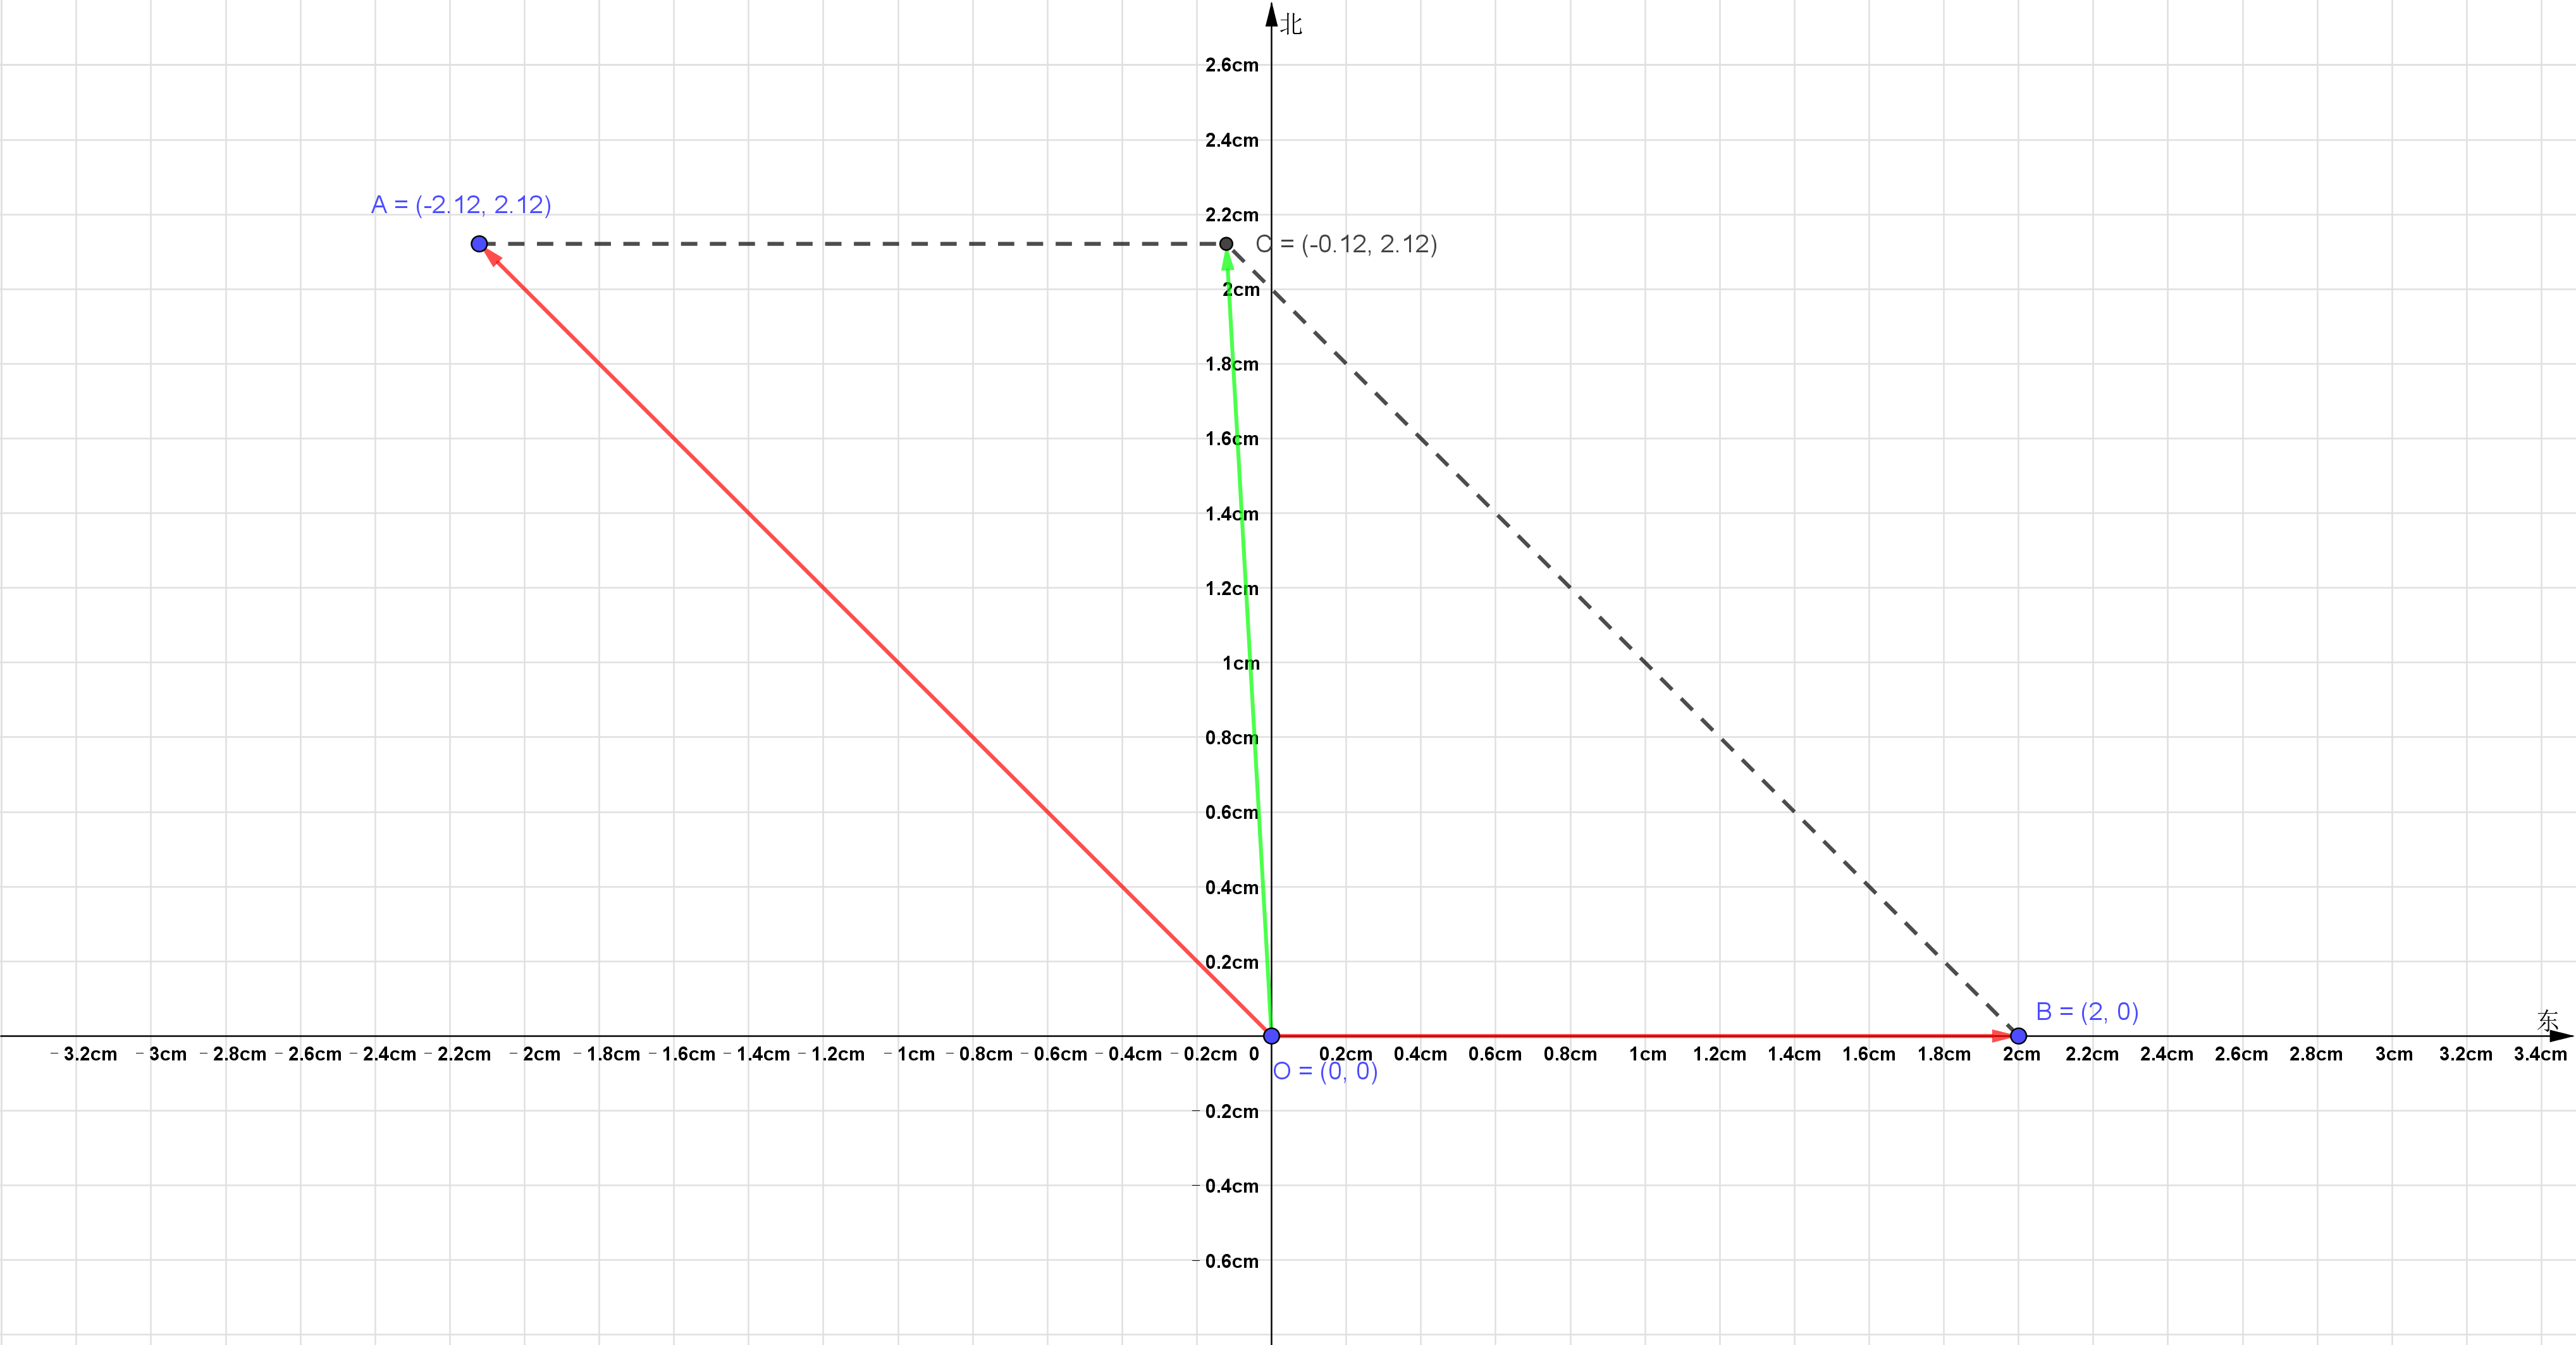
\includegraphics[width=0.7\textwidth]{2_3a.png}
	\label{2_3a}
	\end{minipage}
	}
	\subfloat[]{
	\begin{minipage}[t]{0.5\linewidth}
	\centering
	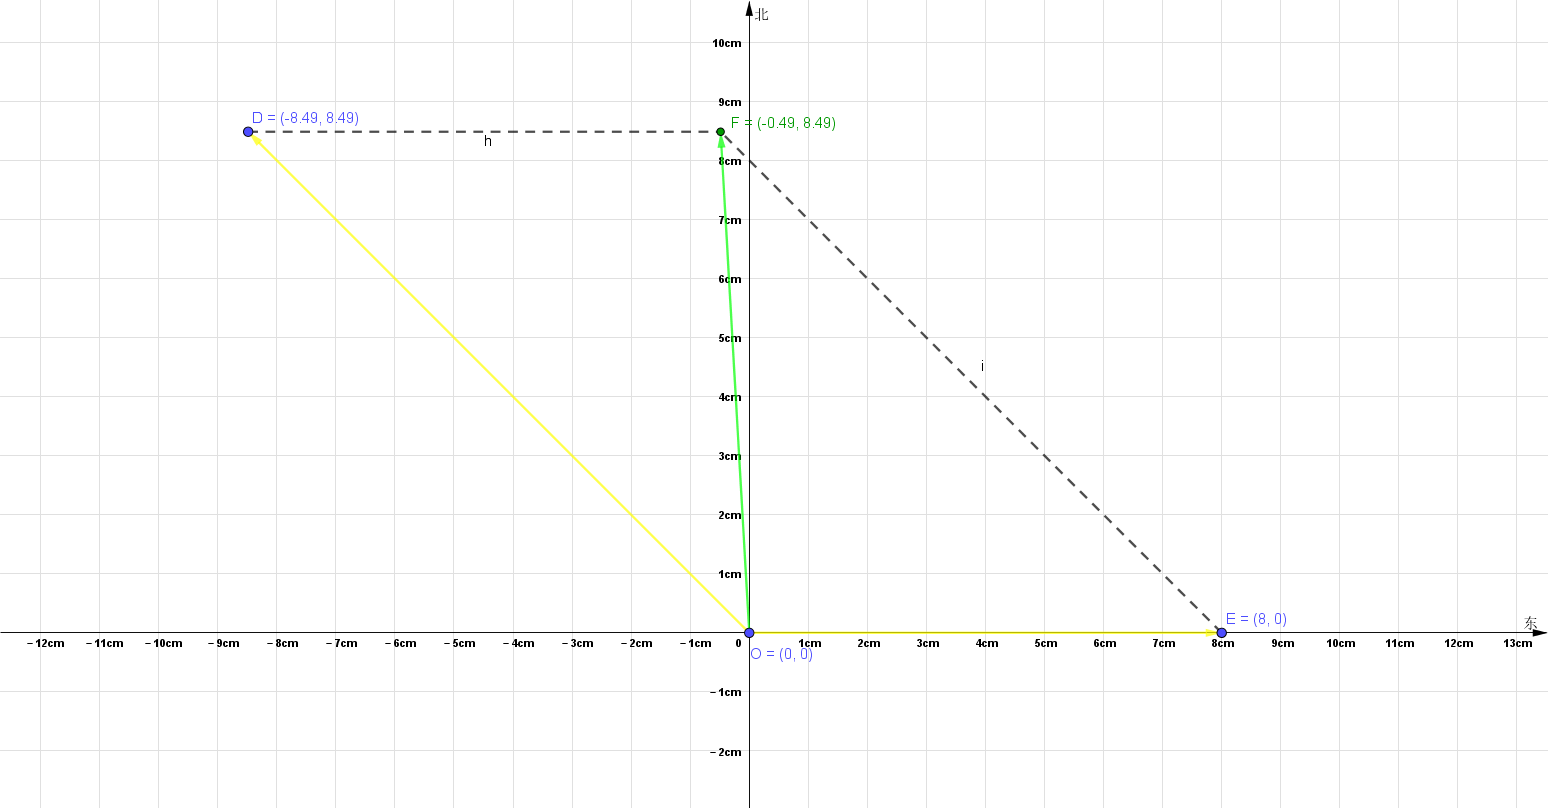
\includegraphics[width=0.7\textwidth]{2_3b.png}
	\label{2_3b}
	\end{minipage}
	}sss
	\\	
	\subfloat[]{
	\begin{minipage}[t]{0.5\linewidth}
	\centering
	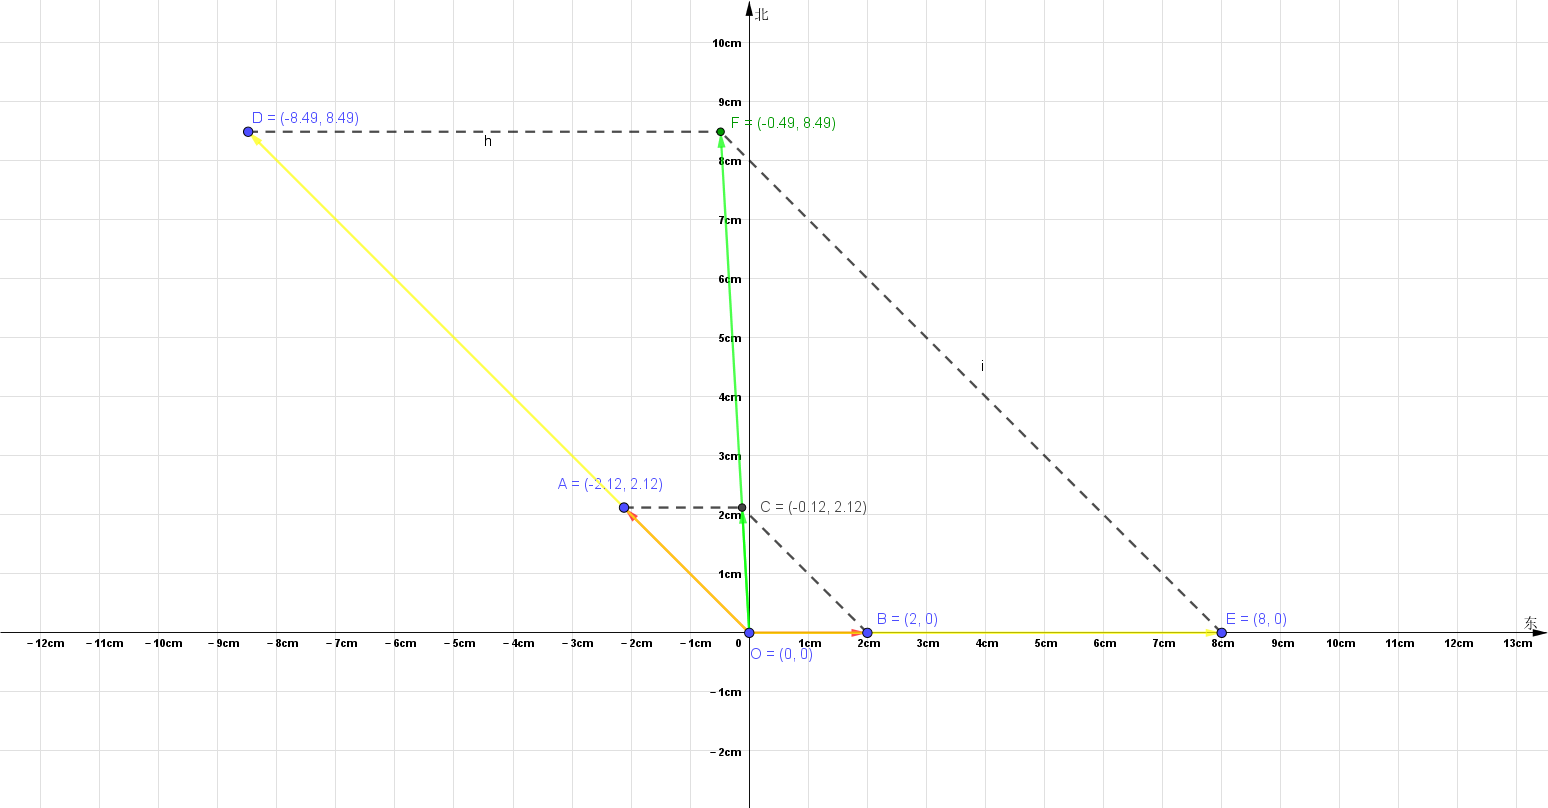
\includegraphics[width=0.7\textwidth]{2_3c.png}
	\label{2_3c}
	\end{minipage}
	}
	\caption{}
	\label{2_3}
\end{figure}
%%%
%%%
%%%
%%%
%%%
\subsection{矢量乘标量}
\begin{enumerate}[(a)]
	\item 如下图(\ref{2_4a})所示。
	\item 如下图(\ref{2_4b})所示。
	\item 如下图(\ref{2_4c})所示。
	\item 根据题意可以知道,矢量$\bm{A}$,$\bm{B}$ 分别为
	\[
	\begin{aligned}
	&\bm{A} = (2 \cos20\degree,2\sin20\degree) \approx  (1.88,0.68),\\
	&\bm{B} = (3.5 \cos40\degree,-3.5\sin40\degree) \approx (2.68,-2.25)
	\end{aligned}
	\]
则,对于(b)小问,
\[
\begin{aligned}
&\bm{C} = -2\bm{A} = (-3.76,-1.37),\bm{D} = 3\bm{B} = (8.04,-6.75)\\
&\bm{E} = \bm{C} + \bm{D} = (4.28,-8.12)
\end{aligned}
\]

对于(c)小问,可以设$ a \bm{A} + b \bm{B} = (0,10) $,则列出如下方程组(\ref{2_4d_e}):
\begin{equation}
\left\{
\begin{aligned}
&aA_x + bB_x = 0 \\
&aA_y + bB_y = 10
\end{aligned}
\right.
\label{2_4d_e}
\end{equation}
解得
\[
\left\{
\begin{aligned}
&a \approx 4.42 \\
&b \approx -3.10
\end{aligned}
\right.
\]
\end{enumerate}

%%%%以下画图时间
\begin{figure}[htbp]
	\centering
	\subfloat[]{
	\begin{minipage}[t]{0.5\linewidth}
	\centering
	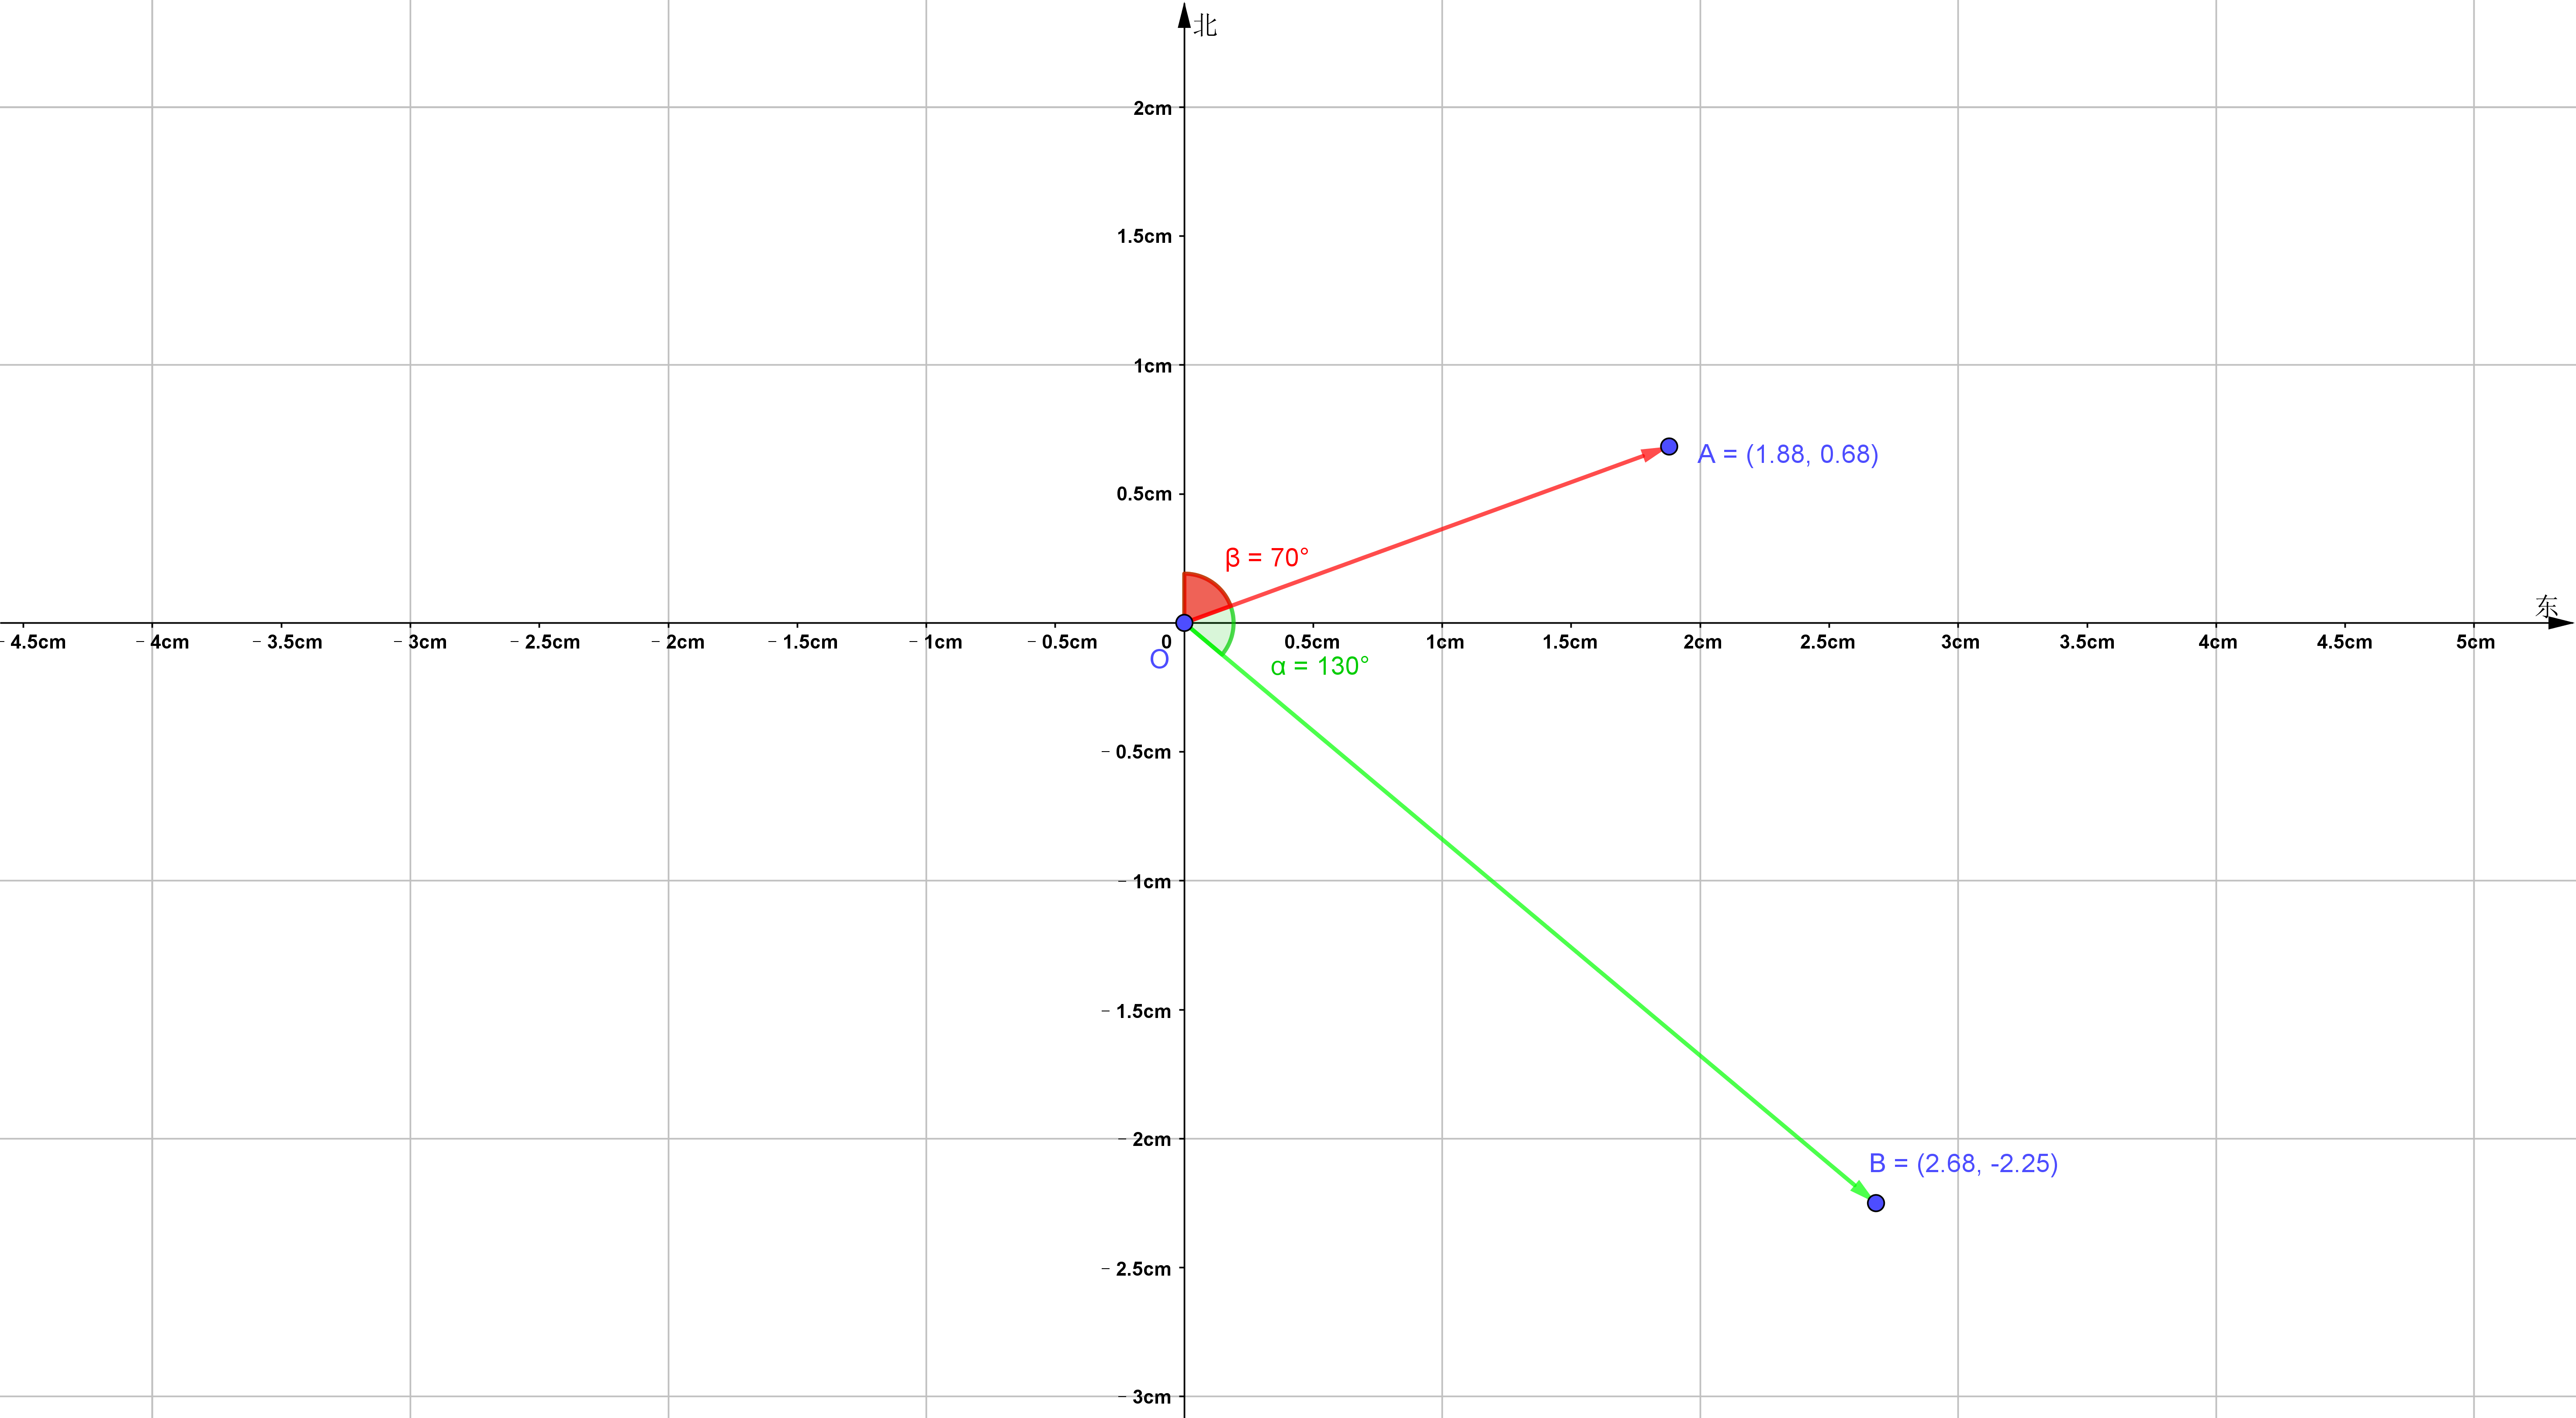
\includegraphics[width=0.7\textwidth]{2_4a.png}
	\label{2_4a}
	\end{minipage}
	}
	\subfloat[]{
	\begin{minipage}[t]{0.5\linewidth}
	\centering
	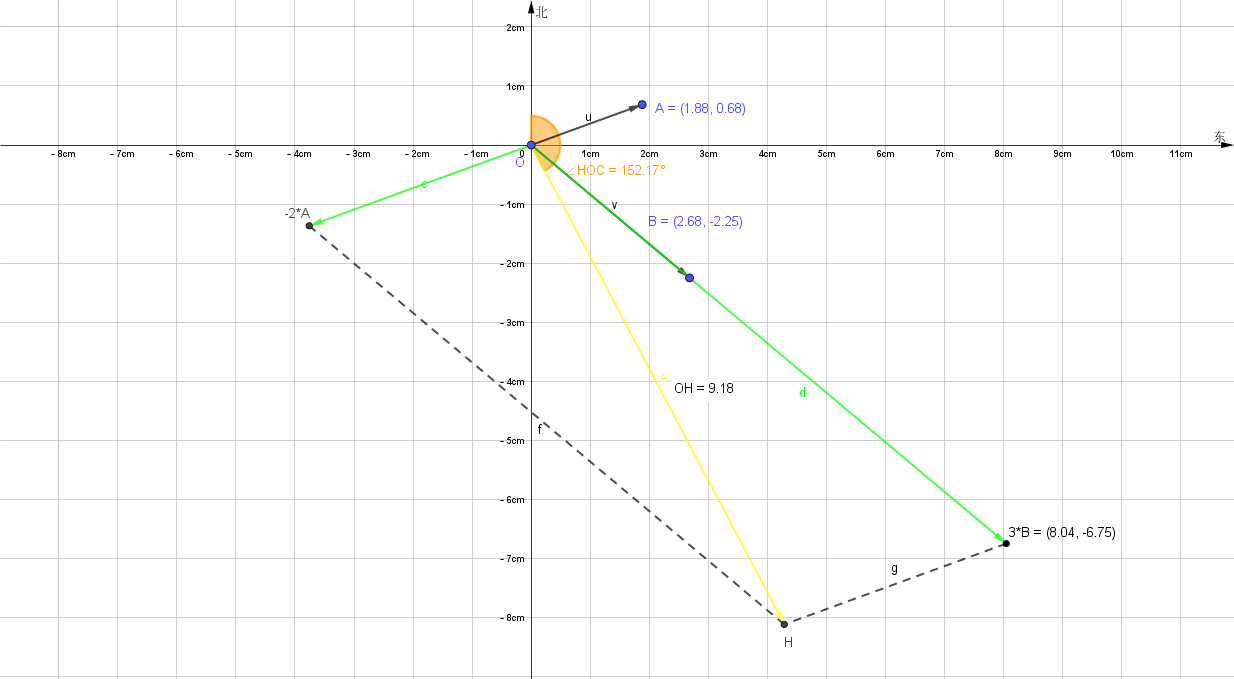
\includegraphics[width=0.7\textwidth]{2_4b.png}
	\label{2_4b}
	\end{minipage}
	}
	\\
	\subfloat[]{
	\begin{minipage}[t]{0.5\linewidth}
	\centering
	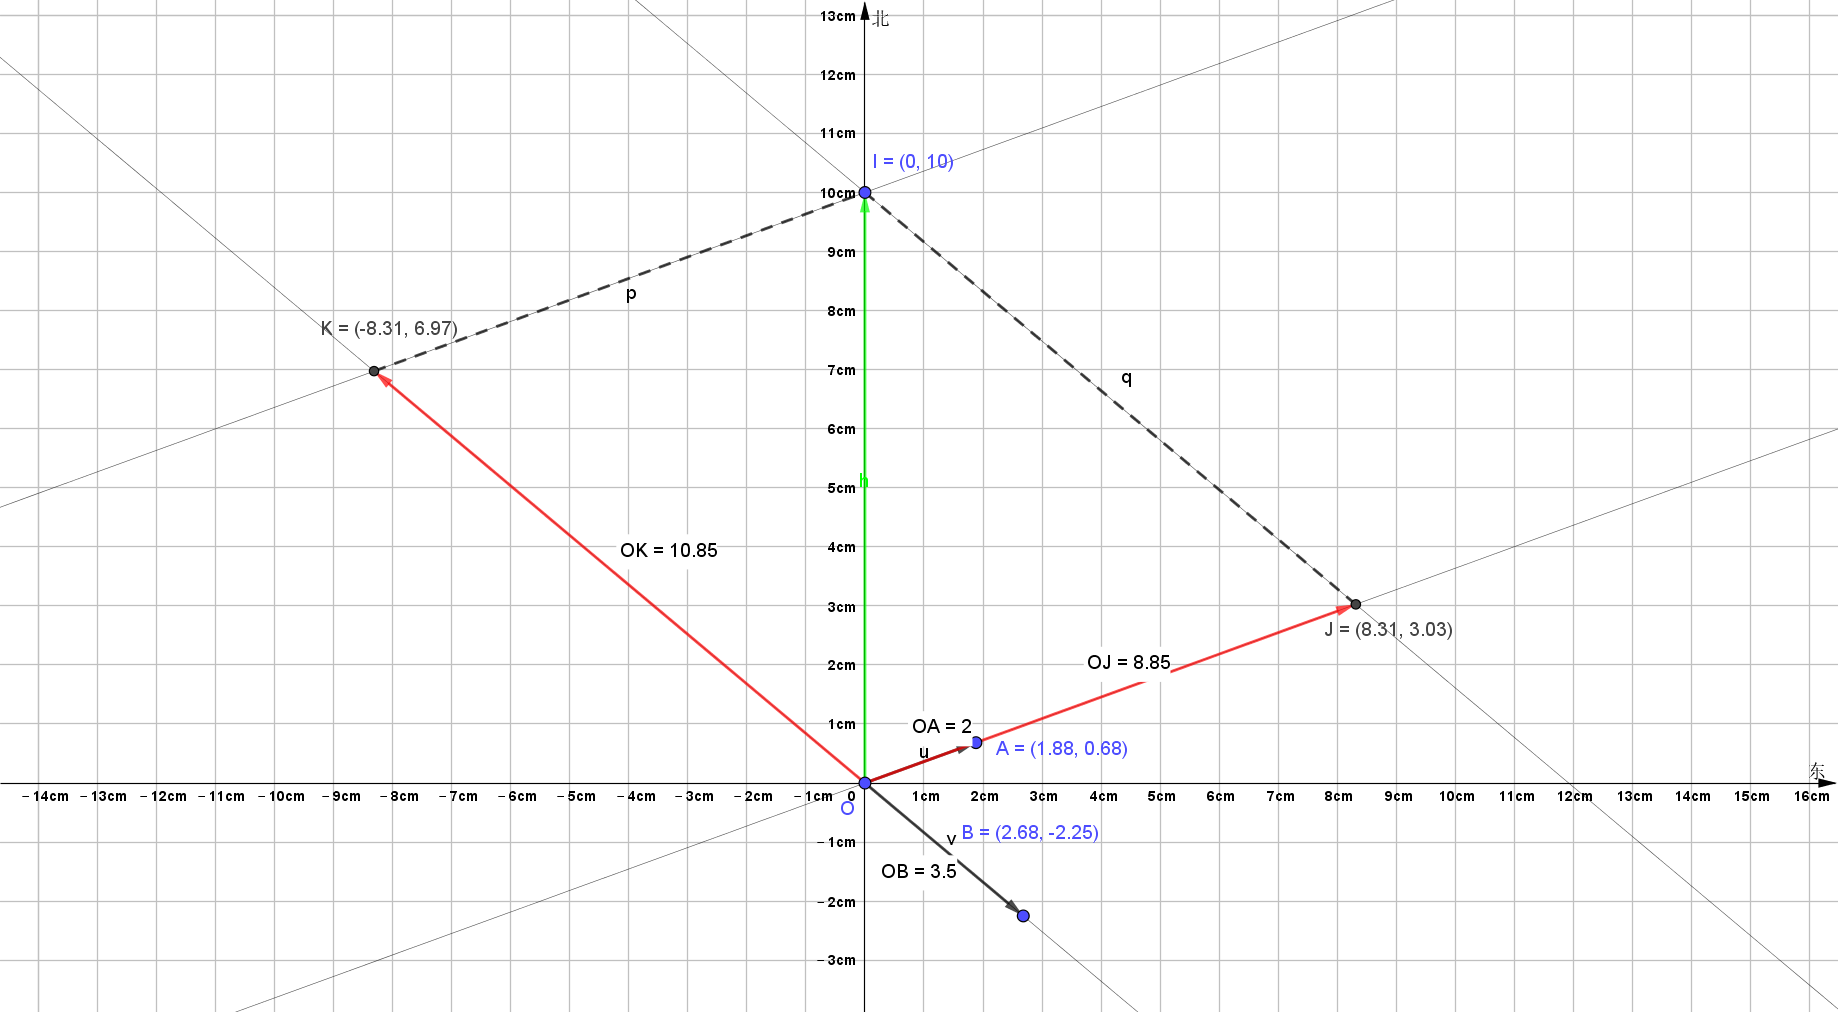
\includegraphics[width=0.7\textwidth]{2_4c.png}
	\label{2_4c}
	\end{minipage}
	}
	\caption{}
	\label{2_4}	
\end{figure}
%%%
%%%
%%%
%%%
%%%
\subsection{二矢量的标量积和矢量积}
\begin{enumerate}[(a)]
%%%%%% 5.1 题  %%%%%%%%%%%%%%	
	\item
	\[
	\begin{aligned}
	&|\bm{a}| = \sqrt{3^2+4^2+(-5)^2} = \sqrt{50} = 5\sqrt{2} \\
	&|\bm{b}| = \sqrt{(-1)^2+2^2+6^2} = \sqrt{41}
	\end{aligned}
	\]
%%%%%% 5.2 题  %%%%%%%%%%%%%%	
	\item
	\[
	\bm{a}\cdot\bm{b} = a_x b_x + a_y b_y + a_z b_z = 3 \cdot (-1) + 4 \cdot 2 + (-5) \cdot 6 =  -5
	\]
%%%%%% 5.3 题  %%%%%%%%%%%%%%	
	\item
	$\bm{a},\ \bm{b}$之间的夹角的余弦值为
	\[
	\cos<\bm{a},\bm{b}> = \frac{\bm{a}\cdot\bm{b}}{|\bm{a}||\bm{b}|} = \frac{-25}{\sqrt{50} \cdot \sqrt{41}} = \frac{-5}{\sqrt{82}} \approx -0.552
	\]
	所以,$\bm{a},\ \bm{b}$之间的夹角为
	\[
	\arccos(\frac{-5}{\sqrt{82}}) \approx 123.52\degree
	\]
%%%%%% 5.4 题  %%%%%%%%%%%%%%	
	\item
	\[
	\begin{aligned}
	&\frac{a_x}{|\bm{a}|} = \frac{3}{5\sqrt{2}},\quad \frac{a_y}{|\bm{a}|} = \frac{4}{5\sqrt{2}}, \quad
	\frac{a_z}{|\bm{a}|} = \frac{-2}{\sqrt{2}} \\
	&\frac{b_x}{|\bm{b}|} = \frac{-1}{\sqrt{41}}, \quad \frac{b_y}{|\bm{b}|} = \frac{2}{\sqrt{41}}, \quad
	\frac{b_z}{|\bm{b}|} = \frac{6}{\sqrt{41}}
	\end{aligned}
	\]
%%%%%% 5.5题  %%%%%%%%%%%%%%	
	\item
	\[
	\begin{aligned}
	&\bm{a} + \bm{b} = (3-1)\bm{\hat{x}} + (4+2)\bm{\hat{y}} + (-5+6)\bm{\hat{z}} = 2\bm{\hat{x}} + 6\bm{\hat{y}} + \bm{\hat{z}} \\
	&\bm{a} - \bm{b} = (3+1)\bm{\hat{x}} + (4-2)\bm{\hat{y}} + (-5-6)\bm{\hat{z}} = 4\bm{\hat{x}} + 2\bm{\hat{y}} -11\bm{\hat{z}}
	\end{aligned}
	\]	
%%%%%% 5.6题  %%%%%%%%%%%%%%
	\item
	\[
	\begin{aligned}
	\bm{a} \times \bm{b}
	& =
	\begin{vmatrix}
		 x & y & z \\
 		3 & 4 & -5 \\
 		-1 & 2 & 6 \\
 	\end{vmatrix} \\
	& = (4 \cdot 6)\bm{\hat{x}} + (-1) \cdot(-5)\bm{\hat{y}} + (3 \cdot 2)\bm{\hat{z}} - \\
	&\quad [(-5 \cdot 2)\bm{\hat{x}} + (3 \cdot 6)\bm{\hat{y}} + (-1 \cdot 4)\bm{\hat{z}}] \\
	& = 34\bm{\hat{x}} - 13\bm{\hat{y}} + 10\bm{\hat{z}}
	\end{aligned}
	\]
\end{enumerate}
%%%
%%%
%%%
%%%
%%%
\subsection{矢量代数}
\begin{enumerate}[(a)]
%%%%%% 6.1题  %%%%%%%%%%%%%%
	\item 因为
	\[
	\begin{aligned}
	(\bm{a} + \bm{b}) + (\bm{a} - \bm{b})
	&= (11+(-5))\bm{\hat{x}} + (-1 + 11)\bm{\hat{y}} + (5+9)\bm{\hat{z}} \\
	&= 6 \bm{\hat{x}} + 10\bm{\hat{y}} + 14\bm{\hat{z}} \\
	&= 2\bm{a}
	\end{aligned}
	\]
	所以
	\[
	\begin{aligned}
	&\bm{a} = 3 \bm{\hat{x}} + 5\bm{\hat{y}} + 7\bm{\hat{z}}  \\
	&\bm{b} = \bm{a} + \bm{b} - \bm{a} = 8 \bm{\hat{x}} - 4\bm{\hat{y}} - 2\bm{\hat{z}}
	\end{aligned}
	\]
%%%%%% 6.2题  %%%%%%%%%%%%%%
	\item
	因为$ \bm{a} $ 与 $ \bm{a} + \bm{b} $ 的夹角的余弦值为
	\[
	\begin{aligned}
	\cos<\bm{a},\bm{b}> &= \frac{\bm{a} \cdot (\bm{a} + \bm{b})}{|\bm{a}||(\bm{a} + \bm{b})|}
						    &=\frac{3 \cdot 11 + (-1) \cdot 5 + 5 \cdot 7}{\sqrt{3^2+5^2+7^2} \cdot \sqrt{11^2+(-1)^2+5^2}} & \approx 0.57
	\end{aligned}
	\]
	所以$ \bm{a} $ 与 $ \bm{a} + \bm{b} $ 的夹角为
	\[
	\arccos(0.57) \approx 55.22\degree
	\]
\end{enumerate}
%%%
%%%
%%%
%%%
%%%
\subsection{速度的矢量加法}
\begin{enumerate}[(a)]
%%%%%% 7.1题  %%%%%%%%%%%%%%
	\item 由题意可以设
	\[
	\begin{aligned}
	&\bm{v_\text{船}} = 2.5\bm{\hat{y}} \\
	&\bm{v_\text{水}} = \bm{\hat{x}}
	\end{aligned}
	\]
	则 $$ \bm{v_\text{实际}} = \bm{v_\text{船}} + \bm{v_\text{水}} = \bm{\hat{x}} +2.5 \bm{\hat{y}} $$
	因此,他实际的前进方向与原定的径直方向的夹角以及速度大小分别为
	\[
	\begin{aligned}
	\arccos(\cos<\bm{v_\text{实际}},\bm{v_\text{船}}>) = \arccos\left(\frac{\bm{v_\text{实际}} \cdot \bm{v_\text{船}}}{|\bm{v_\text{实际}}| |\bm{v_\text{船}}|}\right) = \frac{6.25}{\sqrt{6.25} \cdot \sqrt{7.25}} \approx 68.19\degree \\
	|\bm{v_\text{实际}}| = \sqrt{1^2 + 2.5^2} = \sqrt{7.25} \, \textrm{m/s} \approx 2.69 \, \textrm{m/s}
	\end{aligned}
	\]
%%%%%% 7.2题  %%%%%%%%%%%%%%
	\item 设此人的前进的速度$ \bm{v_0} $ 满足$ \bm{v_0} = a\bm{\hat{x}} + b\bm{\hat{y}} $时,能够与水流垂直的方向前进,前进速度为$ \bm{v_c} = c\bm{\hat{y}} $,则速度$ \bm{v_0} $应当满足
	\[
	\begin{aligned}
	&\bm{v_0} + \bm{v_\text{水}} = \bm{v_c} \\
	\Rightarrow &(a + 1)\bm{\hat{x}} + b\bm{\hat{y}} = c\bm{\hat{y}} \\
	\end{aligned}
	\]
	即
	\[ a = -1,\; b = c. \]
	所以
	\[	\bm{v_0} = - \bm{\hat{x}} + c \bm{\hat{y}}	\]
	前进方向与水流方向的夹角余弦值为
	\[
	\cos(\bm{v_0},\bm{v_\text{水}}) = \frac{\bm{v_0} \cdot \bm{v_\text{水}}}{|\bm{v_0}| |\bm{v_\text{水}}|} = \frac{c-1}{\sqrt{c^2+1}}
	\]
\end{enumerate}

%%%
%%%
%%%
%%%
%%%
\subsection{速度的合成}
设 x 轴正方向为东,y轴正方向为北,则风速$ v_1$ 满足
\[
\bm{v_1} = \sqrt{\frac{30^2}{2}}\bm{\hat{x}} -  \sqrt{\frac{30^2}{2}}\bm{\hat{y}} = 15\sqrt{2}\bm{\hat{x}} - 15\sqrt{2}\bm{\hat{y}}
\]
飞行员满足要求的最终的速度$ \bm{v} $满足
\[
\bm{v} = v\bm{\hat{x}},\; v = \frac{200}{(\frac{40}{60})} \textrm{km/h} = 300 \  \textrm{km/h}
\]
所以,飞行员的飞行速度$ \bm{v_0} $ 应为
\[
\bm{v_0} = \bm{v} - \bm{v_1} = (300 - 15\sqrt{2})\bm{\hat{x}} - 15\sqrt{2}\bm{\hat{y}} \approx 278.78\bm{\hat{x}} + 21.21\bm{\hat{y}}
\]
$ \bm{v_0} $与x轴的夹角$ \alpha $ 为
\[
\alpha = \frac{v_{0x}}{|\bm{v_0}|} = \arccos(\frac{300 - 15\sqrt{2}}{\sqrt{(300 - 15\sqrt{2})^2 + ( - 15\sqrt{2})^2}}) \approx 4.351\degree
\]

若以空气的流动方向为x轴正方向,即将坐标系逆时针旋转$ \frac{\pi}{4} $,则飞行员相当于与流动空气的速度矢量$ \bm{v_{00}} $变为
 \[
 \bm{v_{00}} = |\bm{v_0}|\cos(\alpha + \frac{\pi}{4})\bm{\hat{x}} + |\bm{v_0}|\sin(\alpha + \frac{\pi}{4})\bm{\hat{y}} \approx 182.13\bm{\hat{x}} + 212.13\bm{\hat{y}}
 \]
%%%
%%%
%%%
%%%
%%%

\subsection{矢量运算,相对位置矢量}
\begin{enumerate}[(a)]
%%%%%% 9.1题  %%%%%%%%%%%%%%
	\item
	两个粒子的位置如下图(\ref{2_9a})。粒子2 相对 粒子1的位移$ \bm{r} $ 为
	\[
	\bm{r} = \bm{r_2} - \bm{r_1} = -2\bm{\hat{x}} + 7\bm{\hat{y}} - 3\bm{\hat{z}}
	\]
%%%%%% 9.2题  %%%%%%%%%%%%%%	
	\item
	\[
	\begin{aligned}
	&|\bm{r_1}| = \bm{r_1}\cdot\bm{r_1} = \sqrt{4^2+3^2+8^2} \approx 9.43 \\
	&|\bm{r_2}| = \bm{r_2}\cdot\bm{r_2} = \sqrt{2^2+10^2+5^2} \approx 11.36 \\
	&|\bm{r}| = \bm{r}\cdot\bm{r} = \sqrt{(-2)^2+7^2+(-3)^2} \approx 7.87
\end{aligned}
	\]
%%%%%% 9.3题  %%%%%%%%%%%%%%	
	\item
	设$ \bm{r_1},\;\bm{r_2} $的夹角$ \theta_1 = \arccos(t_1)$,$ \bm{r_1},\;\bm{r} $的夹角$ \theta_2 = \arccos(t_2)$,$ \bm{r_2},\;\bm{r} $的夹角$ \theta_3 = \arccos(t_3)$,则$ t_1,\;t_2,\;t_3 $分别为
	\[
	\begin{aligned}
	&t_1 = \cos<\bm{r_1},\bm{r_2}> = \frac{\bm{r_1}\cdot\bm{r_2}}{|\bm{r_1}| |\bm{r_2}|} =  \frac{8+30+40}{9.43\cdot 11.36} \approx 0.728, \\
	&t_2 =  \cos<\bm{r_1},\bm{r}> = \frac{\bm{r_1}\cdot\bm{r}}{|\bm{r_1}| |\bm{r}|} =  \frac{-8+21-24}{9.43\cdot 7.87} \approx -0.148, \\
	&t_3 =  \cos<\bm{r_2},\bm{r}> = \frac{\bm{r_2}\cdot\bm{r}}{|\bm{r_2}| |\bm{r}|} =  \frac{-4+70-15}{11.36\cdot 7.87} \approx 0.57.
\end{aligned}
	\]
	所以
	\[
	\begin{aligned}
	&\theta_1 = \arccos(0.728) \approx 43.28\degree, \\
	&\theta_2 = \arccos(0.148) \approx 98.51\degree, \\
	&\theta_3 = \arccos(-0.57) \approx 55.25\degree.
\end{aligned}
	\]
%%%%%% 9.4题  %%%%%%%%%%%%%%
	\item
	$ \bm{r} $ 在$ \bm{r_1} $ 上的投影为
	\[
	|\bm{r}|\cos(\theta_2) = \frac{\bm{r} \cdot \bm{r_1}}{|\bm{r_1}|} = \frac{4\cdot(-2) + 3\cdot7 + 8\cdot(-3)}{9.43} = -1.16	
	\]
%%%%%% 9.5题  %%%%%%%%%%%%%%	
	\item
	\[
	\begin{aligned}
	\bm{r_1} \times \bm{r_2} &=
	\begin{vmatrix}
	\bm{\hat{x}} & \bm{\hat{y}} & \bm{\hat{z}} \\
	4 & 3 & 8 \\
	2 & 10 & 5
\end{vmatrix} \\
	&= 15\bm{\hat{x}} + 16\bm{\hat{y}} + 40\bm{\hat{z}} - (80\bm{\hat{x}} + 20\bm{\hat{y}} + 6\bm{\hat{z}}) \\
	&= -65\bm{\hat{x}} - 4\bm{\hat{y}} + 34\bm{\hat{z}}
\end{aligned}
	\]
\end{enumerate}


%%%%以下画图时间
\begin{figure}[htbp]
	\centering
	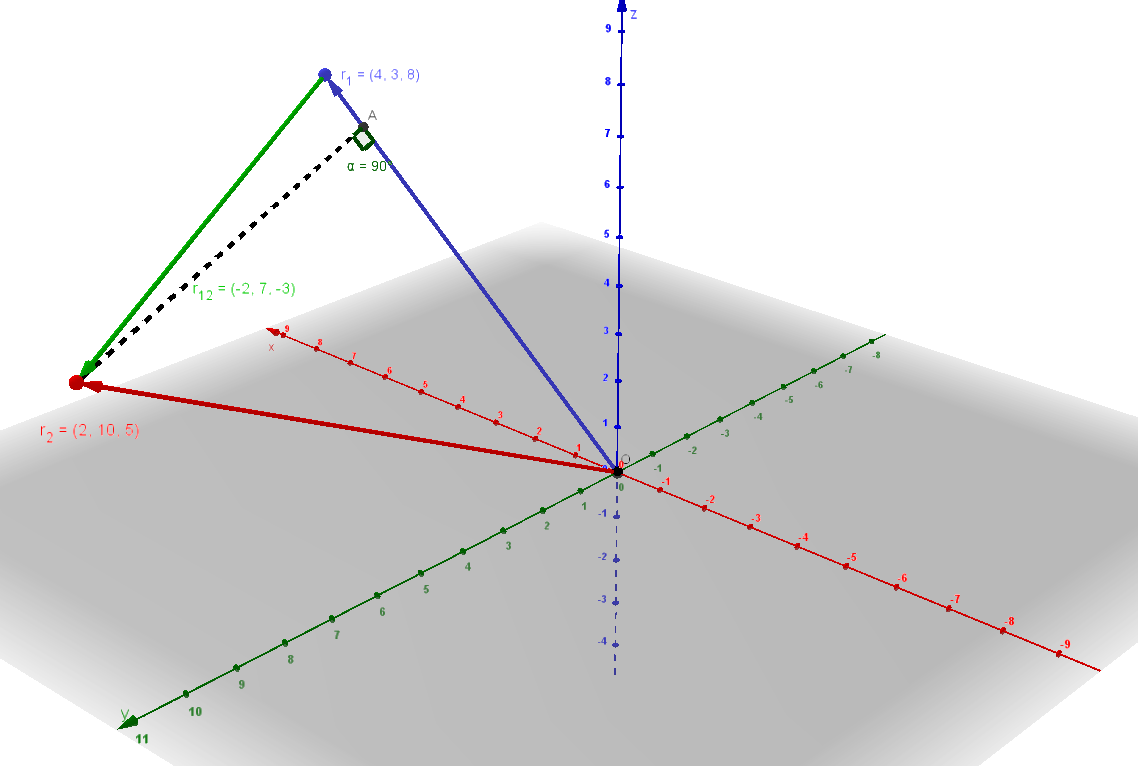
\includegraphics[width=0.7\textwidth]{2_9a.png}
	\caption{}
	\label{2_9a}
\end{figure}
%%%
%%%
%%%
%%%
%%%
\subsection{两个质点最接近的情况}
根据题意,可以设质点1和质点2的位置矢量$ \bm{r_1},\;\bm{r_2}$分别是
\[
\bm{r_1} = (-3 + 2t)\bm{\hat{x}},\; \bm{r_2} = (-3 + 3t)\bm{\hat{y}}
\]
\begin{enumerate}[(a)]
%%%%%% 10.1题  %%%%%%%%%%%%%%	
	\item
	质点2相对质点1的位置矢量$ \bm{r_2} - \bm{r_1} $为
	\[
	\bm{r_2} - \bm{r_1} = (3 - 2t)\bm{\hat{x}} + (-3 + 3t)\bm{\hat{y}}
	\]
%%%%%% 10.2题  %%%%%%%%%%%%%%	
	\item
	当$r = | \bm{r_2} - \bm{r_1} |$取最小值时,两个质点的位置最接近,
	\[
	r = |\bm{r_2} - \bm{r_1}| = (3-2t)^2 + (-3+3t)^2 = 13t^2 - 30t + 18
	\]
	这是以时间t为自变量的二次函数$r(t)$,当$r'(t) = 26t - 30 = 0$,函数有最小值,由此解得$ t = \frac{15}{13}$ s,此时两质点之间的距离$ r = \frac{9}{13}$ cm,质点1的位置$\bm{r_1}$和质点2的位置$\bm{r_2}$分别是
	\[
	\bm{r_1} = \frac{9}{13}\bm{\hat{x}},\;\bm{r_2} = \frac{6}{13}\bm{\hat{y}}
	\]
\end{enumerate}
%%%
%%%
%%%
%%%
%%%
\subsection{立方体的体对角线}
在正方体上建立如图(\ref{2_11})所示的直角坐标系,并选择如图所示的两条体对角线,则相应的顶点O、B、C、D的坐标为(0,0,0)、(1,1,1)、(0,1,0)、(1,0,1),则求两条体对角线的夹角可以变为求矢量$\bm{OB}$和矢量$\bm{CD}$的夹角。
\[
\begin{aligned}
\bm{OB} = (1,1,1),\quad \bm{CD} = (1,-1,1),\\
\cos<\bm{OB},\bm{CD})>= \frac{\bm{OB}\cdot\bm{CD}}{|\bm{OB}| |\bm{CD}|} = \frac{1}{\sqrt{3}\cdot \sqrt{3}} = \frac{1}{3}
\end{aligned}
\]
所以,正方体内两条体对角线的夹角为$\arccos\left(\frac{1}{3}\right)$


%%%%以下画图时间
\begin{figure}[htbp]
	\centering
	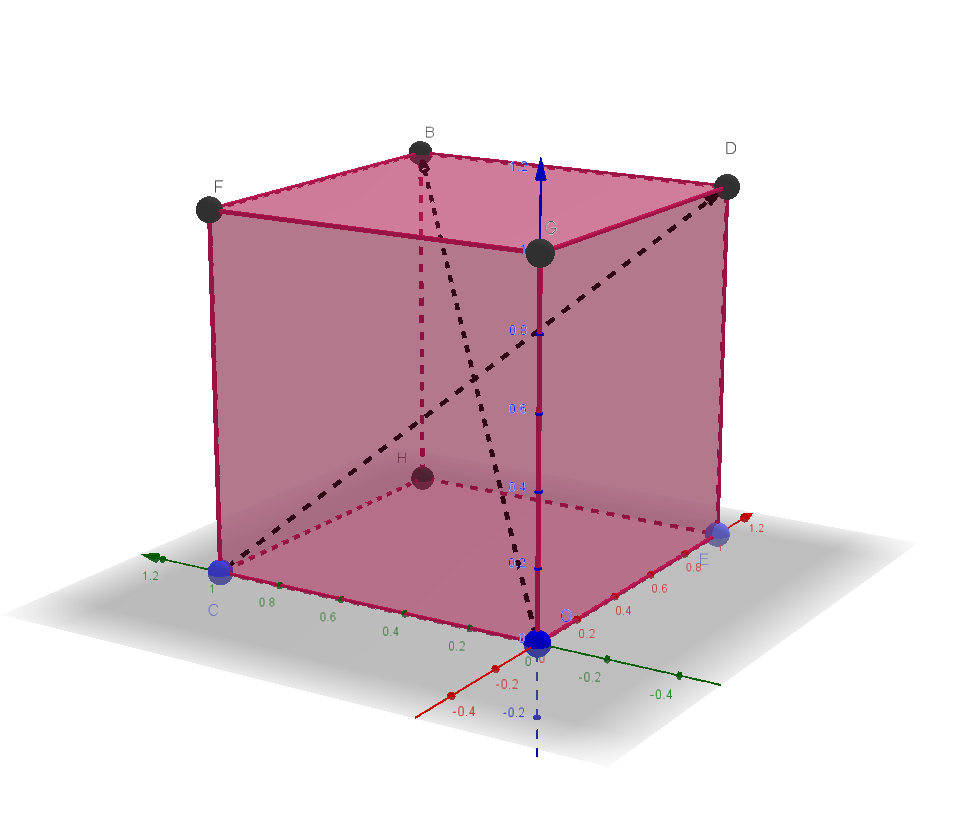
\includegraphics[width=0.7\textwidth]{2_11.png}
	\caption{}
	\label{2_11}
\end{figure}
%%%
%%%
%%%
%%%
%%%
\subsection{$\bm{a}\bot \bm{b}$的条件}
证明:
\[
\begin{aligned}
&\because \quad |\bm{a} + \bm{b}| = |\bm{a} - \bm{b}| \\
&\therefore \quad (\bm{a} + \bm{b})^2 = (\bm{a} - \bm{b})^2 \Rightarrow a^2 + b^2 + 2\bm{a}\cdot\bm{b} - (a^2 + b^2 - 2\bm{a}\cdot\bm{b}) = 0 \\
&\therefore \quad 4\bm{a}\cdot\bm{b} = 0 \rightarrow \bm{a}\cdot\bm{b} = 0 \Leftrightarrow  |a| |b|\cos<a,b> = 0
\end{aligned}
\]
当$ |\bm{a}|=0$ 或者 $|\bm{b}|=0 $,即其中至少有一个为零向量时,$ \bm{a} \bot \bm{b} $恒成立;当$|\bm{a},\;|\bm{b}|$均不为零时,则有$\cos<\bm{a},\bm{b}>=0$,即$\bm{a},\;\bm{b}$之间的夹角为90\degree。

综上,当$\quad |\bm{a} + \bm{b}| = |\bm{a} - \bm{b}|$时,有$\bm{a}\bot \bm{b}$
%%%
%%%
%%%
%%%
%%%
\subsection{平行矢量和垂直矢量}
\[
\begin{aligned}
&\bm{B}\bot\bm{A} \Leftrightarrow \bm{B} \cdot \bm{A} = 0  \Rightarrow 5x + 18 = 0 \Rightarrow x = -\frac{18}{5} \\
&\bm{C}\bot\bm{A} \Leftrightarrow \bm{C} \cdot \bm{A} = 0 \Rightarrow 10 + 6y = 0 \Rightarrow y = -\frac{5}{3} \\
&\because \bm{B} = -\frac{18}{5}\bm{\hat{x}} + 3\bm{\hat{y}} = -\frac{5}{9}(2\bm{\hat{x}} - \frac{5}{3}\bm{\hat{y}}) = -\frac{5}{9}\bm{C} \\
&\therefore \quad \bm{B} \parallel \bm{C}
\end{aligned}
\]
三维空间中,与第三个矢量互相垂直的两个矢量不一定相互平行,如直角坐标系则是相互垂直,也可能是没有任何关系。
%%%
%%%
%%%
%%%
%%%
\subsection{平行六面体的体积}
平行六面体的体积$V$应为
\[
\begin{aligned}
V
& = (\bm{\hat{x}} + 2\bm{\hat{y}})\times4\bm{\hat{y}} \cdot (\bm{\hat{y}} + 3\bm{\hat{z}}) \\
& =
\begin{vmatrix}
\bm{\hat{x}} & \bm{\hat{y}} & \bm{\hat{z}} \\
1 & 2 & 0 \\
0 & 4 & 0
\end{vmatrix}
\cdot  (\bm{\hat{y}} + 3\bm{\hat{z}}) \\
& = 4\bm{\hat{z}} \cdot (\bm{\hat{y}} + 3\bm{\hat{z}}) \\
& = 12
\end{aligned}
\]
%%%
%%%
%%%
%%%
%%%
\subsection{力的平衡}
\begin{enumerate}[(a)]
%%%%%% 15.1题  %%%%%%%%%%%%%%
	\item
	证明:
	因为
	\[
	\bm{F_R} = \bm{F_1} + \bm{F_2} + \bm{F_3} = 0 \Rightarrow
	\bm{F_1} + \bm{F_2} = -\bm{F_3}
	\]
	则两边同时平方,有
	\[
	\bm{F_1}^2 + 2\bm{F_1} \cdot \bm{F_2} + \bm{F_2}^2 = \bm{F_3}^2
	\]
	即
	\[
	\begin{aligned}
	\bm{F_1}^2  + \bm{F_2}^2 - \bm{F_3}^2
	&= - 2\bm{F_1} \cdot \bm{F_2} \\
	&= -2|\bm{F_1}| |\bm{F_2}|\cos<\bm{F_1},\bm{F_2}>  \\
	&= 2|\bm{F_1}| |\bm{F_2}|\cos<\bm{F_1},\bm{F_2}> \\
	&\Rightarrow \cos<\bm{F_1},\bm{F_2}> = \frac{\bm{F_1}^2  + \bm{F_2}^2 - \bm{F_3}^2}{2|\bm{F_1}| |\bm{F_2}|}
\end{aligned}
	\]
	这正是三角形的余弦定理,所以$\bm{F_1},\;\bm{F_2},\;\bm{F_3}$一定构成三角形
%%%%%% 15.2题  %%%%%%%%%%%%%%
	\item
	若题设成立,应有
	\[
	\bm{F_1} \times \bm{F_2} \cdot \bm{F_3} = 0.
	\]
	根据(a)可知,$\bm{F_1},\;\bm{F_2},\;\bm{F_3}$一定构成三角形,即有
	\[
	\bm{F_1} \times \bm{F_2} \cdot \bm{F_3} \ne 0.
	\]
	与题设的推论矛盾,故题设不成立。
%%%%%% 15.3题  %%%%%%%%%%%%%%
	\item
	根据(a)的结论,拉力$bm{T}$,垂直向下的力$\bm{F_{1}}$ 以及需要施加的力$\bm{F_{x}}$构成一个如图(\ref{2_15c})所示的三角形,因此
	\[
	\cos(\beta) = \frac{\bm{F_1}^2  + \bm{T}^2 - \bm{F_x}^2}{2|\bm{F_1}| |\bm{T}|} \approx 0.995.
	\]
	将$ \bm{F_{1}} = 10 $N,$\bm{T} = 15$ N代入上式计算得:
	\[
	\bm{F_x} \approx 5.15\; \textrm{N},\quad
	\cos<\bm{T},\bm{F_x}> = \frac{\bm{F_x}^2  + \bm{T}^2 - \bm{F_1}^2}{2|\bm{F_x}| |\bm{T}|} \approx 0.982.
	\]
\end{enumerate}


%%%%以下画图时间
\begin{figure}[htbp]
	\centering
	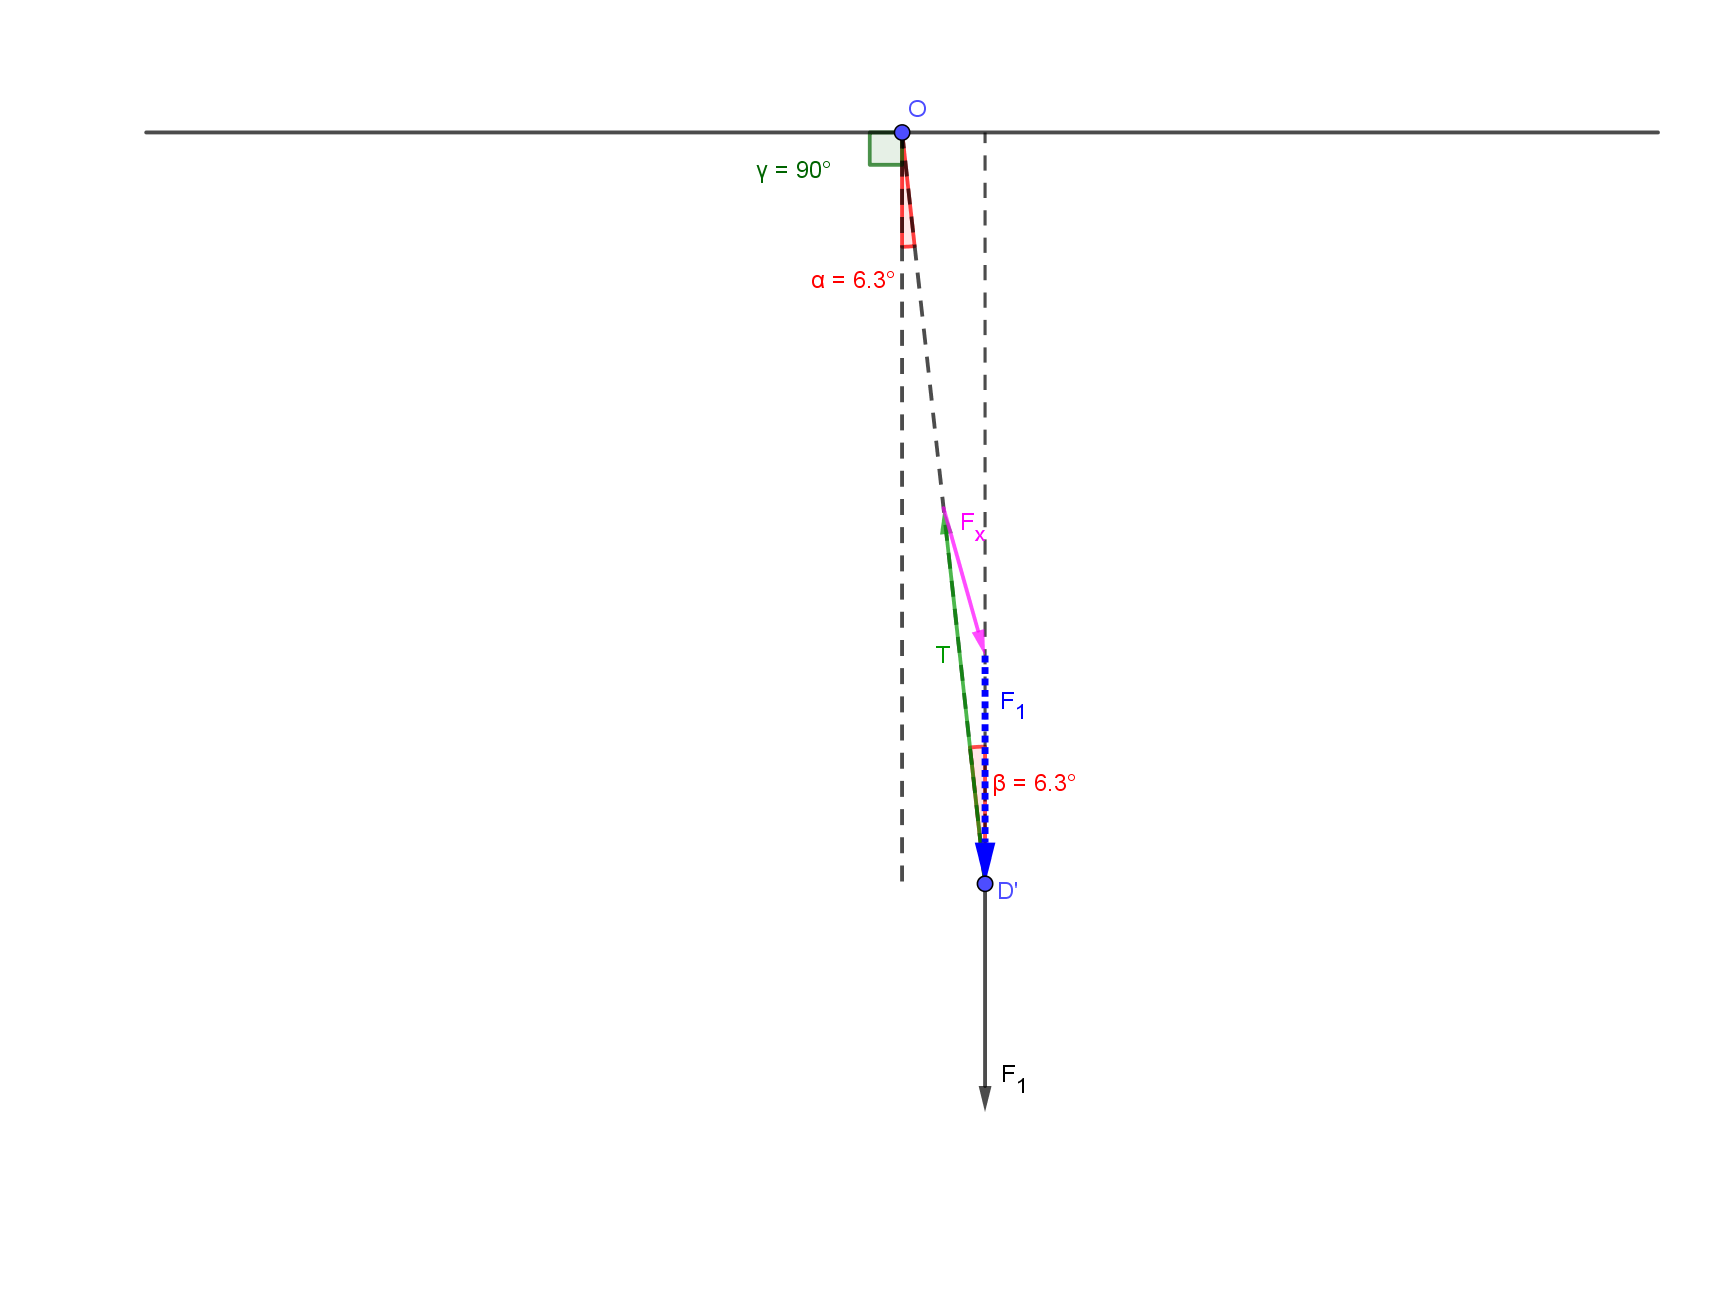
\includegraphics[width=0.7\textwidth]{2_15c.png}
	\caption{}
	\label{2_15c}
\end{figure}
%%%
%%%
%%%
%%%
%%%
\subsection{力所做的功}
\begin{enumerate}[(a)]
%%%%%% 16.1题  %%%%%%%%%%%%%%
	\item
	\[
	\begin{aligned}
	\because \quad
	&\bm{F} = \bm{F_1} + \bm{F_2} = 5\bm{\hat{x}} - 3\bm{\hat{y}} + \bm{\hat{z}}, \\
	&\bm{r_{AB}} = -0.2\bm{\hat{x}} - 0.15\bm{\hat{y}} + 0.07\bm{\hat{z}}, \\
	\therefore \quad
	&W = \bm{F} \cdot \bm{r_{AB}} = (5 \cdot (-0.2) + (-3)\cdot (-5) + 1 \cdot 0.07) \textrm{J} = -0.48\; \textrm{J}.
\end{aligned}
	\]
%%%%%% 16.2题  %%%%%%%%%%%%%%
	\item
	\[
	\begin{aligned}
	W_1 = \bm{F_1} \cdot \bm{r_{AB}} = (1 \cdot (-0.2) + 2 \cdot (-0.15) + 3 \cdot 0.07)\textrm{J} = -0.29\;\textrm{J}, \\
	W_2 = (4 \cdot (-0.2) -5 \cdot (-0.15) -2 \cdot 0.07)\textrm{J} = W - W_1= -0.19\;\textrm{J} .
\end{aligned}
	\]
%%%%%% 16.3题  %%%%%%%%%%%%%%
	\item
	\[
	\begin{aligned}
	&\bm{r_{BA}} =  0.2\bm{\hat{x}} + 0.15\bm{\hat{y}} - 0.07\bm{\hat{z}}, \\
	 &W = \bm{F} \cdot \bm{r_{BA}} = (5 \cdot 0.2 + (-3)\cdot 0.15 + 1 \cdot (-0.07)) \textrm{J} = 0.48\; \textrm{J}
\end{aligned}
	\]
\end{enumerate}
%%%
%%%
%%%
%%%
%%%
\subsection{绕一点的力矩}
\begin{enumerate}[(a)]
%%%%%% 17.1题  %%%%%%%%%%%%%%
	\item
	\[
	\begin{aligned}
	\bm{r} &=  7\bm{\hat{x}} + 3\bm{\hat{y}} + \bm{\hat{z}}, \\
	\bm{N} &= \bm{r} \times \bm{F} \\
	&=
	\begin{vmatrix}
	\bm{\hat{x}} & \bm{\hat{y}} & \bm{\hat{z}} \\
	7 & 3 & 1 \\
	-3 & 1 & 5
	\end{vmatrix} \\
	&= 15\bm{\hat{x}} - 3\bm{\hat{y}} + 7\bm{\hat{z}} - (\bm{\hat{x}} +35 \bm{\hat{y}} - 9\bm{\hat{z}}) \\    &= 14\bm{\hat{x}} - 38\bm{\hat{y}} + 16\bm{\hat{z}}\;(\textrm{N}\cdot\textrm{m}).
\end{aligned}
	\]
%%%%%% 17.2题  %%%%%%%%%%%%%%
	\item
	\[
	\begin{aligned}
	\bm{r_1} &=  7\bm{\hat{x}} + 3\bm{\hat{y}}+\bm{\hat{z}} - 10\bm{\hat{y}} = 7\bm{\hat{x}} -7 \bm{\hat{y}} + \bm{\hat{z}}, \\
	\bm{N} &= \bm{r} \times \bm{F} \\
	&=
	\begin{vmatrix}
	\bm{\hat{x}} & \bm{\hat{y}} & \bm{\hat{z}} \\
	7 & -7 & 1 \\
	-3 & 1 & 5
	\end{vmatrix} \\
	&= -35\bm{\hat{x}} - 3\bm{\hat{y}} + 7\bm{\hat{z}} - (\bm{\hat{x}} +35 \bm{\hat{y}} + 21 \bm{\hat{z}}) \\    &= -36\bm{\hat{x}} - 38\bm{\hat{y}} - 14\bm{\hat{z}}\;(\textrm{N}\cdot\textrm{m}).
\end{aligned}
	\]
\end{enumerate}
%%%
%%%
%%%
%%%
%%%
\subsection{速度和加速度,矢量的微商}
\begin{enumerate}[(a)]
%%%%%% 18.1题  %%%%%%%%%%%%%%
	\item
	\[
	\begin{aligned}
	\bm{v}
	&= \frac{\mathrm{d}\bm{r}}{\mathrm{d}t} \\
	&= \left(\frac{\mathrm{d}16t}{\mathrm{d}t}\bm{\hat{x}} + 16t\frac{\mathrm{d}\bm{\hat{x}}}{\mathrm{d}t}\right) + \left(\frac{\mathrm{d}25t^2}{\mathrm{d}t}\bm{\hat{y}} + 25t^2\frac{\mathrm{d}\bm{\hat{y}}}{\mathrm{d}t}\right) +  \left(\frac{\mathrm{d}33}{\mathrm{d}t}\bm{\hat{z}} + 33\frac{\mathrm{d}\bm{\hat{z}}}{\mathrm{d}t}\right) \\
	&= 16\bm{\hat{x}} + 50t\bm{\hat{y}}, \\
	\bm{a}
	&= \frac{\mathrm{d}\bm{v}}{\mathrm{d}t} = 50\bm{\hat{y}}.
\end{aligned}
	\]
%%%%%% 18.2题  %%%%%%%%%%%%%%
	\item
	\[
	\begin{aligned}
	\bm{v}
	&= \frac{\mathrm{d}\bm{r}}{\mathrm{d}t} = 150\cos(15t)\bm{\hat{x}} + 35\bm{\hat{y}} + 6e^{6t}\bm{\hat{z}}, \\
	\bm{a}
	&= \frac{\mathrm{d}\bm{v}}{\mathrm{d}t} = -2250\sin(15t)\bm{\hat{x}} + 36e^{6t}\bm{\hat{z}}.
\end{aligned}
	\]
\end{enumerate}
%%%
%%%
%%%
%%%
%%%
\subsection{随机运动}
\textcolor{red}{\bfseries{不会做!}}

\textcolor{red}{可以参考《费曼物理学讲义(新千年版)第$ \; 1 \; $卷》第 6 章的$ \S $ 6-3 无规行走。}
%%%
%%%
%%%
%%%
%%%
\subsection{不变性}
\begin{enumerate}[(a)]
%%%%%% 20.1题  %%%%%%%%%%%%%%
	\item
	如下图(\ref{2_20a})所示,
	\[
	\begin{aligned}
	&\bm{\hat{x'}} = |\bm{\hat{x'}}|\cos(\theta)\bm{\hat{x}} + |\bm{\hat{x'}}|\sin(\theta)\bm{\hat{y}} = \cos(\theta)\bm{\hat{x}} + \sin(\theta)\bm{\hat{y}},\\
	&\bm{\hat{y'}} = -|\bm{\hat{y'}}|\sin(\theta)\bm{\hat{x}} + |\bm{\hat{y'}}|\cos(\theta)\bm{\hat{y}} =
	- \sin(\theta)\bm{\hat{x}} + \cos(\theta)\bm{\hat{y}}.
\end{aligned}
	\]
%%%%%% 20.2题  %%%%%%%%%%%%%%
	\item
	\[
	\begin{aligned}
	&\because \quad
	\begin{aligned}
	\bm{A}
	&= A'_x\bm{\hat{x'}} + A'_y\bm{\hat{y'}} + A'_z\bm{\hat{z'}},\\
	&=A'_x(\cos(\theta)\bm{\hat{x}} + \sin(\theta)\bm{\hat{y}}) + A'_y(- \sin(\theta)\bm{\hat{x}} + \cos(\theta)\bm{\hat{y}}) + A'_z\bm{\hat{z}}. \\
\end{aligned} \\
	&\therefore \quad
	\left\{
	\begin{aligned}
	&A'_x\cos(\theta) - A'_y\sin(\theta) = A_x, \\
	&A'_x\sin(\theta) + A'_y\cos(\theta) = A_y, \\
	&A'_z = A_z
\end{aligned}
	\right.
\end{aligned}
	\]
%%%%%% 20.2题  %%%%%%%%%%%%%%
	\item
	\[
	\begin{aligned}
	\because \quad
	&A_x^2 = {A'_x}^2\cos\theta^2 - 2A'_xA'_y\sin\theta\cos\theta + {A'_y}^2\sin\theta^2, \\
	&A_y^2 = {A'_x}^2\sin\theta^2 + 2A'_xA'_y\sin\theta\cos\theta + {A'_y}^2\cos\theta^2, \\
	&A_z^2 = {A'_z}^2. \\
	\therefore \quad
	&A_x^2 + A_y^2 + A_z^2 ={ A'_x}^2(\cos\theta^2 + \sin\theta^2) +  {A'_y}^2(\cos\theta^2 + \sin\theta^2) + {A'_z}^2 = {A'_x}^2 +{ A'_y}^2 +{ A'_z}^2
\end{aligned}
	\]
\end{enumerate}


%%%%以下画图时间
\begin{figure}[htbp]
	\centering
	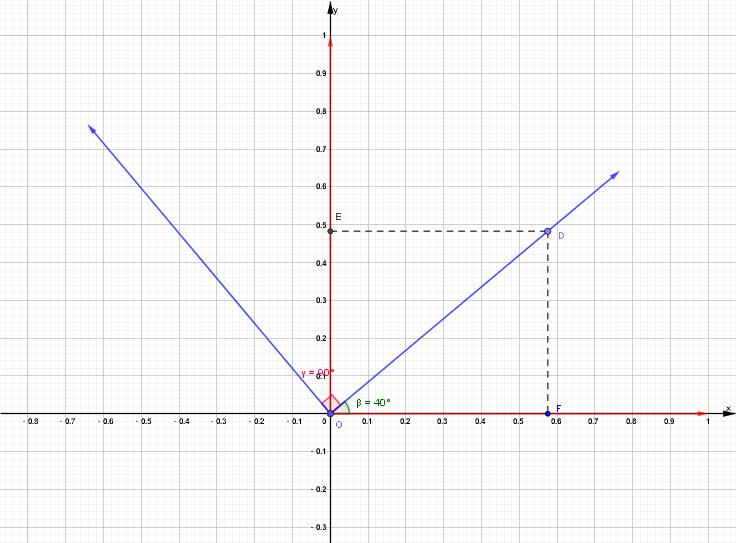
\includegraphics[width=0.7\textwidth]{2_20a.png}
	\caption{}
	\label{2_20a}
\end{figure}
%%%
%%%
%%%
%%%
%%%
\subsection{数学附录}
\subsubsection{对时间的微商,速度和加速度}
\subsubsection{角度}
\subsubsection{函数$\bm{e^x}$}
\subsubsection{级数展开}
\subsubsection{矢量与球极坐标}







\clearpage
%!TeX root =main.tex
%!TEX program = XeLaTeX
% !Mode:: "TeX:UTF-8"

\section{牛顿运动定律}

\subsection{牛顿第三定律}
\begin{enumerate}[(a)]
%%%%%%  1.1 题  %%%%%%%%%%%%%%
	\item
	他可以一只脚放松,另一只脚用力向后蹬,整个人就可以向前滑动,持续这样,就可以到达边缘。
%%%%%%  1.2 题  %%%%%%%%%%%%%%
	\item
	当脚向后蹬的时候,学生给了地面一个向后下方的作用力$\bm{F}$,根据“牛顿第三定律”,地面也会给学生一个相等大小,但是方向向前的作用力$\bm{F_1} = -\bm{F}$。根据“牛顿第二定律”,质量为$m$的学生在$\bm{F_1}$的作用下得到一个加速度$\bm{a_1} = \frac{\bm{F_1}}{m}$,开始向边缘运动,而地面也会有一个加速度$\bm{a} = \frac{\bm{F}}{M}$,因为$M \to \infty$,所以$\bm{F} \to 0$,所以地面没动,人向边缘滑去。
\end{enumerate}
%%%
%%%
%%%
%%%
%%%
\subsection{}
\label{subsec_3.2}
{\bfseries 证明1:}设O点与P点的水平距离为$x$,P点离地面高度为$y$,子弹速度为$\bm{v}$,$\bm{v}$与水平方向的夹角为$\theta$,重力加速度为$\bm{g}$,则子弹飞过距离$x$ 所需的时间$t$满足
\[
t = \frac{x}{v_x} = \frac{x}{v\sin\theta} = \frac{x}{v \frac{x}{\sqrt{x^2+y^2}}}
\]
在这段时间$t$内,靶体在做自由落体运动,子弹在做竖直上抛运动,靶体距离地面的高度$h$,子弹离地面的高度$H$分别满足
\[
\begin{aligned}
& h = y-\frac{1}{2}gt^2, \\
& H = v_yt - \frac{1}{2}gt^2
\end{aligned}
\]
因为枪是瞄准P点的,因此,子弹初速度的水平分量$v_x$和竖直分量$v_y$满足关系
\[
\frac{v_y}{v_x} = \frac{y}{x}
\]
将$t,\;v_x,\;v_y$分别代入$h,\,\;H$的表达式中,得到
\[
h = y-\frac{1}{2}g \frac{x^2+y^2}{v^2} = H
\]
即无论子弹的速度$\bm{v}$取值为多少,恒有$h = H$。

{\bfseries 证明2:}我们以靶体为参考系,此时,子弹与靶体间不存在相对加速度,两者的相对运动变为:子弹以速度$\bm{v}$匀速飞向静止的靶体。因此,只要子弹瞄准靶体,最终两者会相遇。
%%%
%%%
%%%
%%%
%%%
\subsection{接球游戏的顶棚高度}
因为球的运动轨迹是开口向下的抛物线,根据题意,孩子们能完成这个游戏的充分条件是抛物线的顶点不能超过顶棚(如下图(\ref{3_3a})所示)。
%%%%以下画图时间
\begin{figure}[htbp]
	\centering
	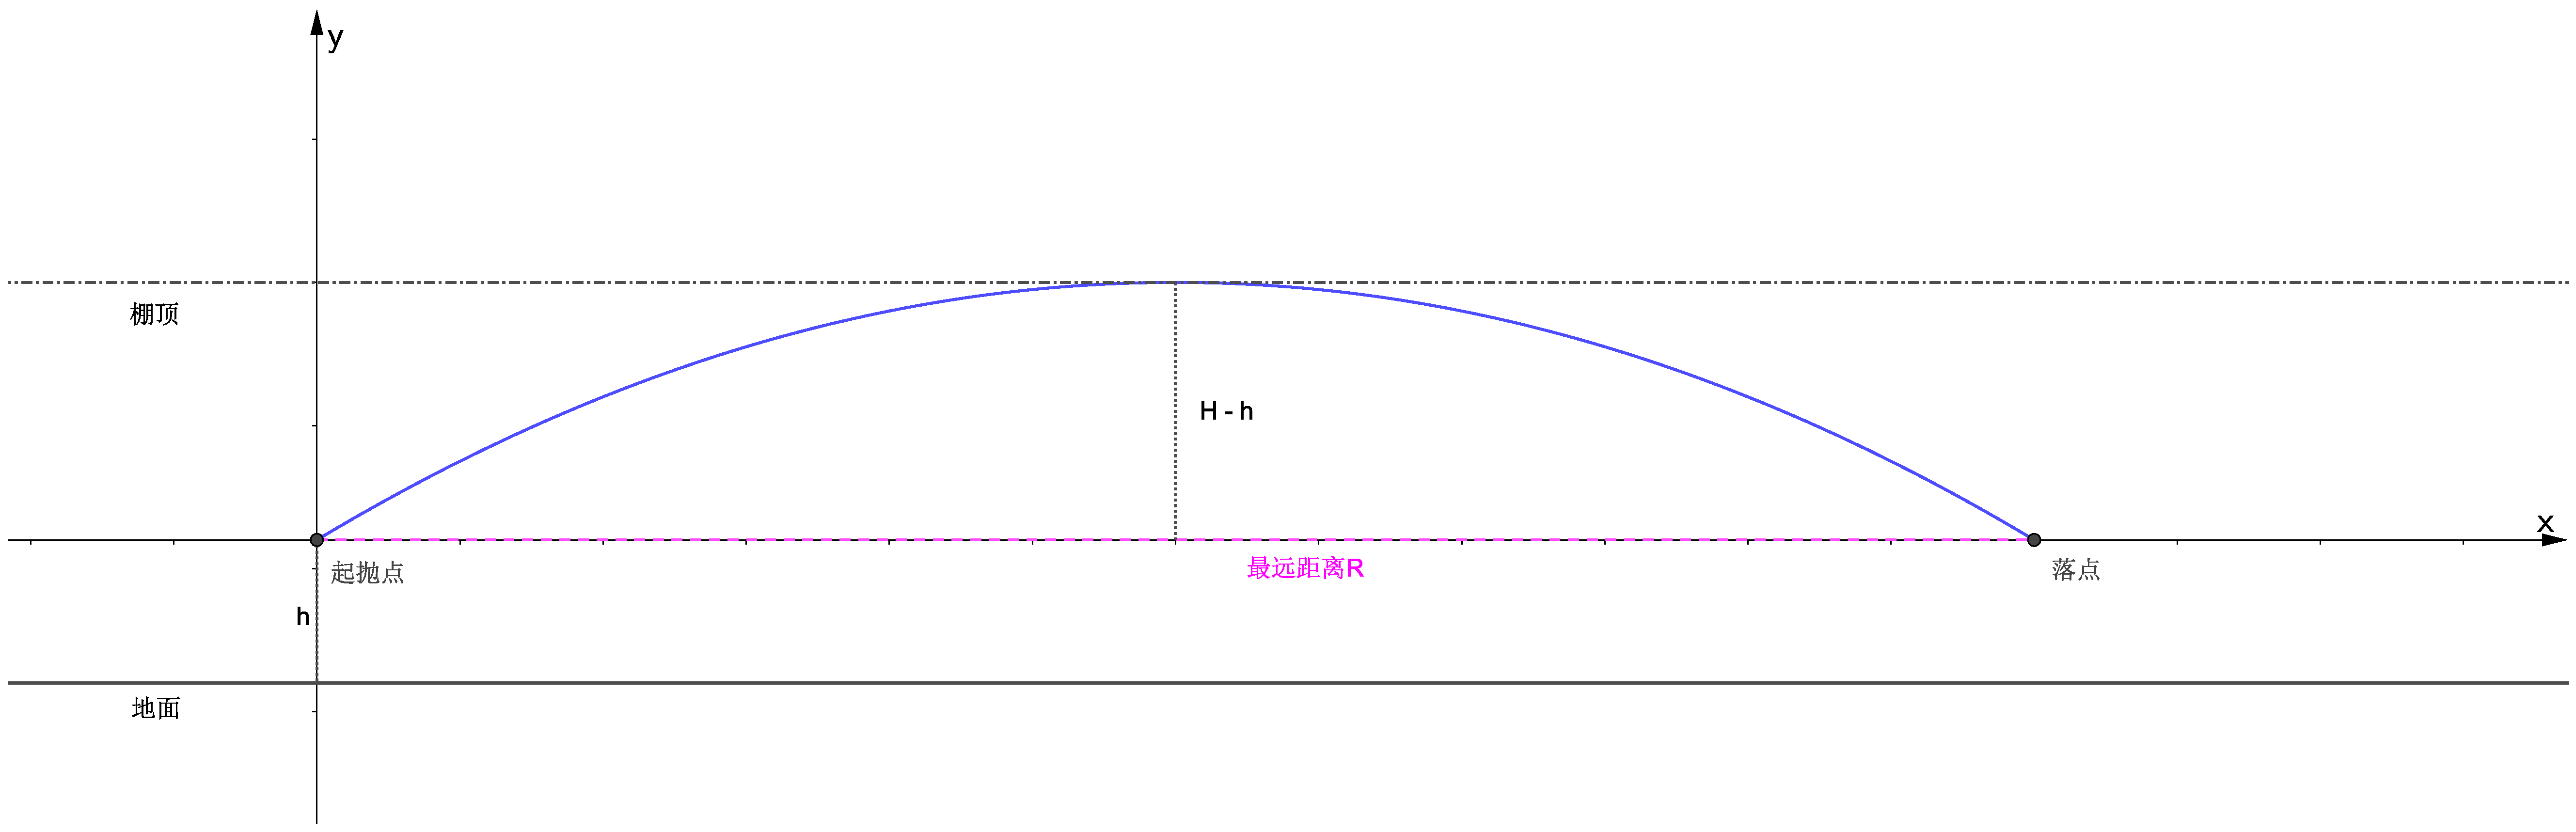
\includegraphics[width=0.8\textwidth]{3_3a.eps}
	\caption{}
	\label{3_3a}
\end{figure}

\noindent
而抛体的运动函数为
\[
y - \left(y_0 + \frac{v_0^2\sin\theta}{2g}\right) = - \frac{g}{2v_0^2\cos^2\theta}\left[x - \left(x_0 + \frac{v_0^2\sin	\theta \cos\theta}{g}\right)\right]^2.
\]
这条抛物线的顶点在
\[
\begin{aligned}
&x_1 = x_0 + \frac{v_0^2\sin \theta\cos \theta}{g}\;, \\
&y_1 = y_0 + \frac{v_0^2 \sin^2 \theta}{2g}\;.
\end{aligned}
\]

不妨建立如图(\ref{3_3a})所示的直角坐标系,假设两个孩子相距的最远距离为$R$,孩子扔球的初始速度大小为$v_0$,与地面的夹角为$\theta$,则有$(x_0, y_0) = (0, 0),\;(x_1,y_1) = (\frac{R}{2},H-h)$,将这些条件代入上述的顶点公式中有:
\[
\begin{aligned}
&\frac{R}{2} = \frac{v_0^2\sin \theta\cos \theta}{g}\;, \\
&H-h = \frac{v_0^2 \sin^2 \theta}{2g}\;.
\end{aligned}
\]

\newpage
\noindent
{\bfseries 解法一(错误解法):}\par
设$l = \sqrt{\frac{R}{2}^2 +(H-h)^2}$,则
\[
\begin{aligned}
&\sin \theta = \frac{H-h}{l}\;, \\
&\cos \theta = \frac{(\frac{R}{2})}{l} = \frac{R}{2l}\;,\\
& \sin 2\theta = 2\sin \theta \cos \theta = \frac{(H-h)R}{l^2}.
\end{aligned}
\]
因此,{\bfseries\textcolor{red}{!!!此处出现矛盾,书上给出的参考答案是第二种。}}
\[
\begin{aligned}
&R = \frac{v_0^2}{g}\frac{(H-h)R}{l} \Rightarrow R = 4\sqrt{\frac{v_0^2}{g}(H-h) - (H-h)^2}\;,\\
&H-h = \frac{v_0^2}{2g}\left(\frac{H-h}{l}\right)^2 \Rightarrow R = 4\sqrt{\frac{v_0^2}{2g}(H-h) - (H-h)^2}\;.
\end{aligned}
\]
{\bfseries\textcolor{red}{警告!!!这种解法有问题!如图(\ref{3_3b})所示,其中的错误是在:将球抛出的初始速度与水平方向的夹角和最高点与最远距离的中点的夹角混淆了!}}


%%%%以下画图时间
\begin{figure}[htbp]
	\centering
	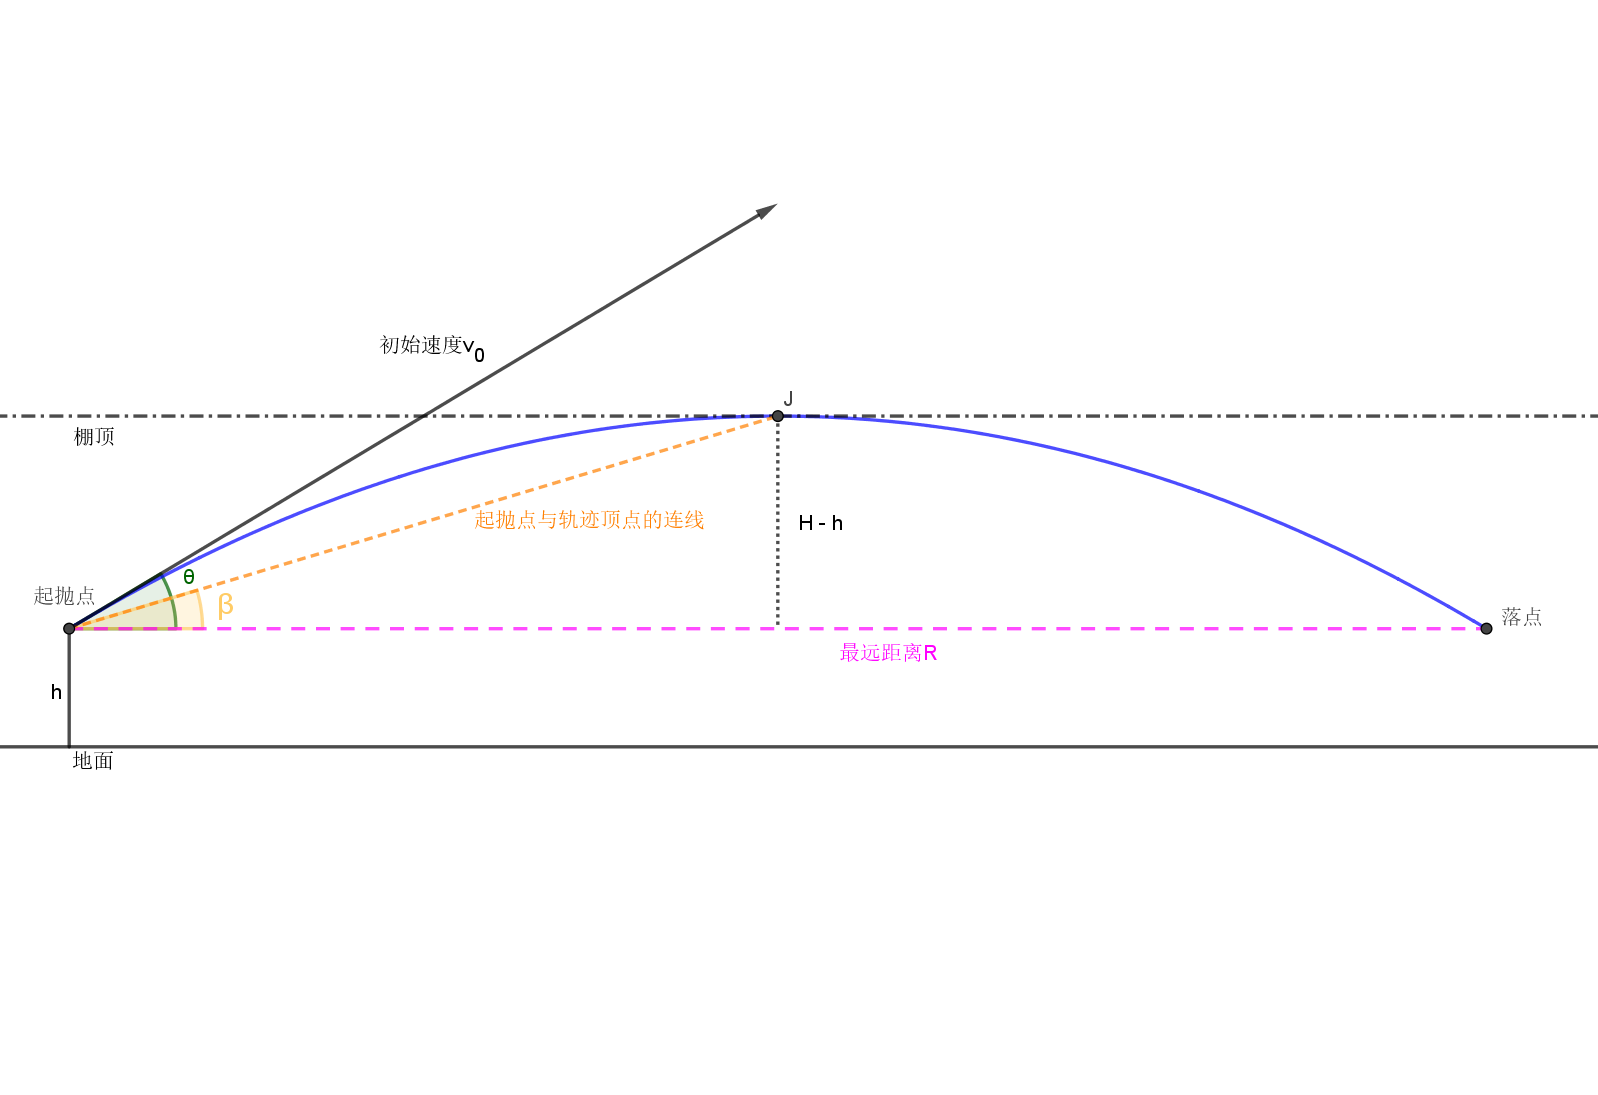
\includegraphics[width=0.8\textwidth]{3_3b.png}
	\caption{}
	\label{3_3b}
\end{figure}

\newpage
\noindent
{\bfseries 解法二:}\par
如图(\ref{3_3c})所示,

%%%%以下画图时间
\begin{figure}[htbp]
	\centering
	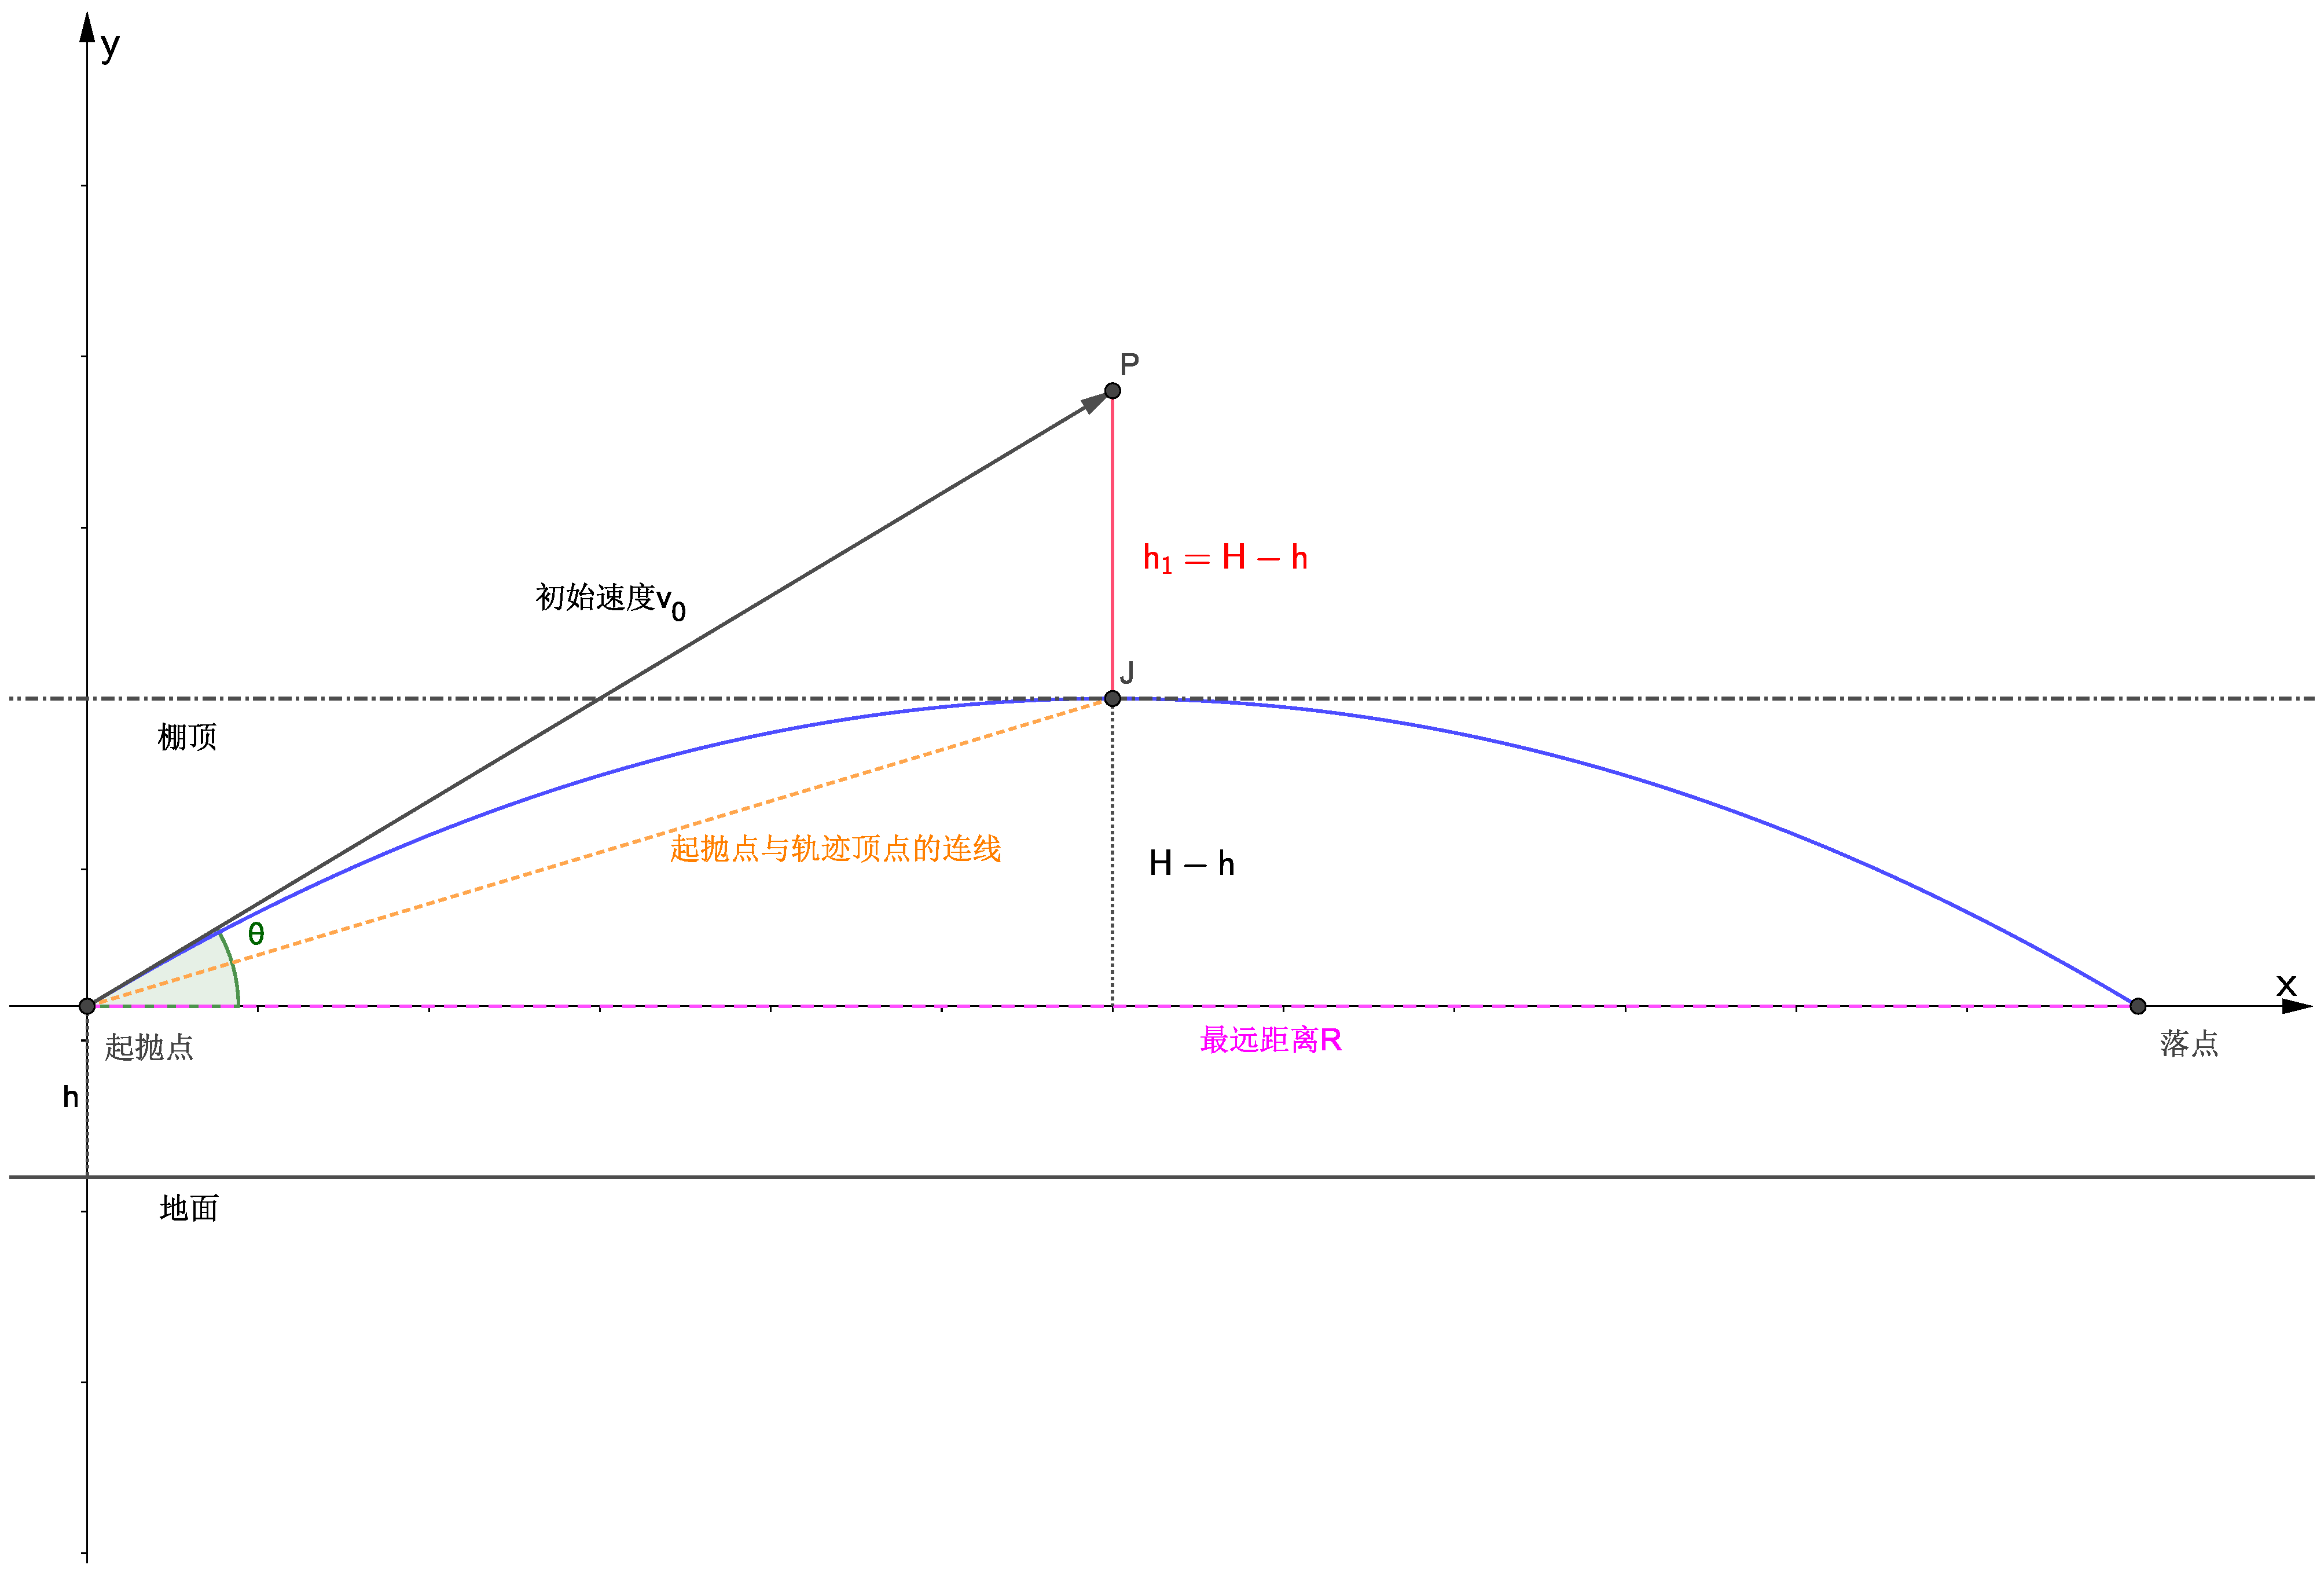
\includegraphics[width=0.8\textwidth]{3_3c.eps}
	\caption{}
	\label{3_3c}
\end{figure}

\noindent
根据运动公式
\[
\begin{aligned}
& 0 - v_y = -gt\;,\\
& 0^2 - v_y^2 = 2g(H-h)
\end{aligned}
\]
可以得到
\[
v_y = gt = \sqrt{2g(H-h)} \Rightarrow t = \sqrt{\frac{2(H-h)}{g}}
\]
根据{\bfseries 题\ref{subsec_3.2}}可以知道,当物体1以任意速度开始做斜上抛运动时,如果在初始速度的方向上有物体2立刻做自由落体运动,那么最终两个物体会在物体1的抛物线轨迹上相遇。由此我们可以知道,图(\ref{3_3c})中,点P到抛物线的顶点J的距离$l_{\text{PJ}}$应该满足
\[
l_{\text{PJ}} = \frac{1}{2}gt^2 = \frac{g}{2} \cdot \frac{2(H-h)}{g} = H - h
\]
由此我们可以得到
\[
\begin{aligned}
& \sin \theta = \frac{2(H - h)}{\sqrt{[2(H - h)]^2 + (\frac{R}{2})^2}}\;,\\
& \cos \theta = \frac{(\frac{R}{2})}{\sqrt{[2(H - h)]^2 + (\frac{R}{2})^2}}\;.
\end{aligned}
\]
将得到的$\sin \theta\;,\cos \theta$分别代入开始得到$R$和$H - h$的表达式中得到
\[
\begin{aligned}
& R = \frac{2v_0^2}{g} \cdot \frac{(H-h)R}{[2(H - h)]^2 + (\frac{R}{2})^2} \Rightarrow R = 4\sqrt{\frac{v_0^2}{2g}(H-h) - (H-h)^2}\;,\\
& H-h = \frac{v_0^2}{2g} \cdot \left(\frac{2(H - h)}{\sqrt{[2(H - h)]^2 + (\frac{R}{2})^2}}\right)^2 \Rightarrow R = 4\sqrt{\frac{v_0^2}{2g}(H-h) - (H-h)^2}\;.
\end{aligned}
\]

\noindent
对于第2问,令$h_0 = H - h$,则
\[
\begin{aligned}
& R = 4\sqrt{\frac{v_0^2}{2g}h_0 - h_0^2}\;,\\
& R' = \frac{\mathrm{d}R}{\mathrm{h_0}} = 4\times \frac{1}{2}\frac{1}{\sqrt{\frac{v_0^2h_0}{2g} - h_0^2}}(\frac{v_0^2}{2g} - 2h_0)\;.
\end{aligned}
\]
令$R'(h_0) = 0$,可以解得$h_0 = \frac{v_0^2}{4g}$,此时$R$有最大值
\[
R = 4\sqrt{ \frac{v_0^2}{2g}\cdot\frac{v_0^2}{4g} - ( \frac{v_0^2}{4g})^2} = \frac{v_0}{g}
\]
此处$R$的最大值表示,在不受棚顶高度限制的情况下孩子在以速度$v_0$将球抛出时所能达到的最远距离,因此$h_0 = H - h$ 表示,在没有棚顶高度限制,并且球达到最远距离的情况下球所能达到的最大高度。
%%%
%%%
%%%
%%%
%%%
\subsection{向上发射}
\begin{enumerate}[(a)]
%%%%%% 4.1题  %%%%%%%%%%%%%%
	\item
	设子弹最高可以到达的高度是$h$,子弹速度为$v$,重力加速度$g = 10\;\text{m/s}^2$,,则
	\[
		\begin{aligned}
			&0 - v = -gt \Rightarrow t = \frac{v}{g} = 3\,\text{s}\;,\\
			&h = vt - \frac{1}{2}gt^2 = 30 \times 3 - 0.5 \times 10 \times 3^2 = 45\;\text{m}\;.
		\end{aligned}
	\]
	因为子弹上升和下降的过程是对称的,因此,每一颗子弹在空中停留的时间均为6s,不妨设此人在$t = 0\,\text{s}$时射出第一发子弹,则在$t = 6\,\text{s}$时这一颗子弹刚好回到地面。根据题意,此人每隔一秒发射一颗子弹,因此,最终(第6秒之后)空中子弹数量为6,在第6秒之前,子弹数量逐渐增加,如下表(\ref{3_3ta})所示。
	\begin{table}[htbp]
		\centering
		\begin{tabular}{c|cccccccccc}
		\hline
		\text{时间/s} & 0 & 1 & 2 & 3 & 4 & 5 & 6 & 7 & ... & n \\
		\hline
		\text{子弹数量/颗} & 1 & 2 & 3 & 4 & 5 & 6 & 6 & 6 & ... & 6 \\
		\hline
		\end{tabular}
		\caption{}
		\label{3_3ta}
	\end{table}
%%%%%% 4.2题  %%%%%%%%%%%%%%
	\item 
	当第一颗子弹b1(在第0秒发射)开始下落时,首先遇到的是在第1秒发射的子弹b2。在此之前,b1运动时间为3s,刚好到达轨迹最高点并开始转做自由落体运动,b2运动时间为$t_2 = 2$s,仍在以速度$v_20$竖直上抛的过程中,以此为时间参考点,因为运动过程对称,因此两者相遇时速度大小为$v_2$,相遇的时间$t_{02}$满足
	\[
		\begin{aligned}
			& v_{20} - v = -gt_2 \\
			& v_2 - v_{20} = -gt_{02} \\
			& -v_2 = -gt_{02}
		\end{aligned}
	\]
	解得:
	\[
		t_{02} = \frac{v-2g}{2g} = 0.5\;\text{s}
	\]
	因此,b1和b2相遇的地方离地面高度$h_2 =h - \frac{1}{2}gt_{02}^2 = 43.75$m。
	b1接下来遇到的子弹是在第2秒发射的子弹b3,在第3秒发射的子弹b4,在第4秒发射的子弹b5,在第5秒发射的子弹b6,根据上面一样的做法,可以分别得到各自相遇的时间和离地面的高度。结果如下表(\ref{3_3tb})所示。
	\begin{table}[htbp]
		\centering
		\begin{tabular}{|c|c|c|c|c|c|c|}
		\hline
		\text{与b1相遇的子弹} & b2 & b2 & b3 & b4 & b5 & b6 \\
		\hline
		\text{时间/s} & 0.5 & 1 & 1.5 & 2 & 2.5 & 3 \\
		\hline
		\text{离地面高度/m} & 43.75 & 40 & 33.75 & 25 & 13.75 & 0 \\
		\hline
		\end{tabular}
		\caption{}
		\label{3_3tb}
	\end{table}
\end{enumerate}
%%%
%%%
%%%
%%%
%%%
\subsection{两个斜面上的摩擦}
设$M_1$受到的重力为$G_1 = M_1g$,摩擦力为$f_1 = \mu_1 G_1\cos \theta_1$,$M_2$受到的重力为$G_2 = M_2g$,摩擦力为$f_2 = \mu_2 G_2\cos \theta_2$,绳子拉力为$T$。
\begin{enumerate}[(a)]
%%%%%% 5.1题  %%%%%%%%%%%%%%	
	\item 
	当$M_1$刚要沿平面下滑时,分别对$M_1$和$M_2$进行受力分析,可以知道,$M_1$刚要下滑,摩擦力和运动趋势相反,即沿斜面向上;而对于$M_2$,因为$M_1$已经要开始滑动,所以$M_2$的状态应当是被$M_1$拉着将要向上走,因此$M_2$的摩擦力是沿斜面向下,所以可以有以下关系:
	\[
		\begin{aligned}
			f_1 & = G_1\sin \theta_1 - T \;,\\
			f_2 & = T - G_2\sin \theta_2
		\end{aligned}
		\]
	将相关的表达式代入后将两式相加,并整理可得:
	\[
		\frac{M_1}{M_2} = \frac{\mu_2\cos\theta_2 + \sin\theta_2}{\sin\theta_1 - \mu_1\cos\theta_1}
		\]
	这就是在条件“$M_1$刚要沿平面下滑时”各个物理量之间要满足的关系。
%%%%%% 5.2题  %%%%%%%%%%%%%%
	\item
	当当$M_2$刚要沿平面下滑时,可以对$M_1$和$M_2$分别进行跟题(a)一样的受力分析,并得出以下关系:
	\[
		\begin{aligned}
			f_1 & = T - G_1\sin \theta_1 \;,\\
			f_2 & = G_2\sin \theta_2 - T
		\end{aligned}
		\]
	将相关的表达式代入后将两式相加,并整理可得:
	\[
		\frac{M_1}{M_2} = \frac{\mu_2\cos\theta_2 - \sin\theta_2}{\sin\theta_1 + \mu_1\cos\theta_1}
		\]
	这就是在条件“$M_2$刚要沿平面下滑时”各个物理量之间要满足的关系。
\end{enumerate}

%%%%以下画图时间




%%%
%%%
%%%
%%%
%%%
\subsection{摩擦力不等于$\mu Mg$}
\begin{enumerate}[(a)]
	\item
	根据题意有
	\[
		F\sin \theta < \mu (Mg + F\cos\theta) \Rightarrow \sin\theta - \mu \cos\theta < \frac{\mu Mg}{F}
		\]
	令$f(\theta) = \sin\theta - \mu \cos\theta, (0 \leqslant \theta \leqslant \frac{\pi}{2})$,则$f'(\theta) = \cos\theta + \mu \sin\theta > 0$恒成立,即$f(\theta)$在定义域内是单调递增的,最大值
	\item
	1+1
\end{enumerate}
%%%
%%%
%%%
%%%
%%%
\subsection{摩擦力不等于$\mu Mg$}
%%%
%%%
%%%
%%%
%%%
\subsection{摩擦力不等于$\mu Mg$}
%%%
%%%
%%%
%%%
%%%
\subsection{摩擦力不等于$\mu Mg$}
%%%
%%%
%%%
%%%
%%%
\subsection{摩擦力不等于$\mu Mg$}
%%%
%%%
%%%
%%%
%%%
\subsection{摩擦力不等于$\mu Mg$}
%%%
%%%
%%%
%%%
%%%
\subsection{摩擦力不等于$\mu Mg$}


\end{document}


